\documentclass[10pt,a4paper,twoside,openright,titlepage,fleqn,%
               headinclude,,footinclude,BCOR5mm,%
               numbers=noenddot,cleardoublepage=empty,%
               tablecaptionabove]{scrbook}
\usepackage[dutch,polutonikogreek,british]{babel}
\usepackage[utf8]{inputenc}
\usepackage[LGRx,T1]{fontenc}
\usepackage[final]{microtype}
\usepackage{amsmath,amssymb,amsthm}
\usepackage{varioref}
\usepackage{hyperref}
\usepackage[style=philosophy-modern,hyperref,backref,square,natbib,ibidtracker=false]{biblatex}
\usepackage[tight,british]{minitoc}
\usepackage{wrapfig}
\usepackage{chngpage}
\usepackage{calc}
\usepackage{mflogo}
\usepackage{caption,listings,graphicx,subfig}
\usepackage{multicol}
\usepackage{makeidx}
\usepackage{xspace}
\usepackage{mparhack}
\usepackage{fixltx2e}
\usepackage[xindy,toc]{glossaries}
\usepackage{relsize}
\usepackage{lipsum}
\usepackage[eulerchapternumbers,subfig,beramono,eulermath,pdfspacing,listings]{classicthesis}
\usepackage{guit}
\usepackage{arsclassica}
\usepackage{enumitem}
\usepackage{graphicx}
\usepackage{tikz}
\usetikzlibrary{automata,positioning,shapes.multipart}
\usepackage{pstricks,pst-node,pst-text,pst-3d}
\usepackage{float}
\usepackage{setspace}
\usepackage{etoolbox}
\usepackage{listings}
\usepackage{tabularx}
%% initialisation
% ********************************************************************
% classicthesis-preamble
% ********************************************************************

\newcommand{\myName}{Xavier Goas Aguililla\xspace}
\newcommand{\myTitle}{A corpus-based approach to the language of the papyri\xspace}
%\newcommand{\mySubTitle}{Methodological questions and select topics\xspace}
\newcommand{\myLocation}{Leuven\xspace}
\newcommand{\myUni}{KU Leuven\xspace}
\newcommand{\myFac}{Faculty of Arts\xspace}
\newcommand{\myDegree}{Master of Arts in de taal- en letterkunde\xspace}
\newcommand{\myProf}{dr. T. Van Hal\xspace}
\newcommand{\myDepartment}{Department of Greek Studies\xspace}

\newcommand{\myTime}{June 2012\xspace}

% ********************************************************************
% hyperref
% ******************************************************************** 
\hypersetup{%
    colorlinks=true, linktocpage=true, pdfstartpage=1, pdfstartview=FitV,%
    breaklinks=true, pdfpagemode=UseNone, pageanchor=true, pdfpagemode=UseOutlines,%
    plainpages=false, bookmarksnumbered, bookmarksopen=true, bookmarksopenlevel=1,%
    hypertexnames=true, pdfhighlight=/O,%
    urlcolor=webbrown, linkcolor=RoyalBlue, citecolor=RoyalBlue, pagecolor=RoyalBlue,%
% uncomment the following line if you want to have black links (e.g., for printing)
% urlcolor=Black, linkcolor=Black, citecolor=Black, pagecolor=Black,%
    pdftitle={\myTitle},%
    pdfauthor={\textcopyright\ \myName},%
    pdfsubject={},%
    pdfkeywords={},%
    pdfcreator={pdfLaTeX},%
    pdfproducer={LaTeX con hyperref e ClassicThesis}%
}

\hypersetup{citecolor=webgreen}
\hypersetup{hyperfootnotes=false,pdfpagelabels}


\newcommand{\mail}[1]{\href{mailto:#1}{\texttt{#1}}}



% ********************************************************************
% caption
% ********************************************************************
\captionsetup{format=hang,font=small}
\captionsetup[table]{skip=\medskipamount} 


% ********************************************************************
% makeidx, multicol
% ********************************************************************
\let\orgtheindex\theindex
\let\orgendtheindex\endtheindex
\def\theindex{%
	\def\twocolumn{\begin{multicols}{2}}%
	\def\onecolumn{}%
	\clearpage
	\orgtheindex
}
\def\endtheindex{%
	\end{multicols}%
	\orgendtheindex
}

\makeindex

% ********************************************************************
% listings
% ********************************************************************

\definecolor{lightergray}{gray}{0.99}

\lstset{language=[LaTeX]Tex,
    keywordstyle=\color{RoyalBlue},
    basicstyle=\normalfont\ttfamily,
    commentstyle=\color{Emerald}\ttfamily,
    stringstyle=\rmfamily,
    numbers=none,
    numberstyle=\scriptsize,
    stepnumber=5,
    numbersep=8pt,
    showstringspaces=false,
    breaklines=true,
    frameround=ftff,
    frame=lines,
    backgroundcolor=\color{lightergray}
}

\lstset{morekeywords=%
        {RequirePackage,newboolean,DeclareOption,setboolean,%
        ProcessOptions,PackageError,ifthenelse,boolean,%
        chapterNumber,sodef,textls,allcapsspacing,%
        MakeTextLowercase,orgtheindex,endtheindex,%
        @ifpackageloaded,undefined,sfdefault,%
        DeclareRobustCommand,spacedallcaps,%
        microtypesetup,MakeTextUppercase,lowsmallcapsspacing,%
        lowsmallcapsspacing,spacedlowsmallcaps,
        spacedlowsmallcaps,lehead,headmark,color,%
        headfont,partname,thepart,titleformat,part,
        titlerule,chapter,thechapter,thesection,%
        subsection,thesubsection,thesubsubsection,%
        paragraph,theparagraph,descriptionlabel,titlespacing,%
        graffito,lineskiplimit,finalhyphendemerits,%
        colorbox,captionsetup,labelitemi,%
        myincludegraphics,hypersetup,setlength,%
        definecolor,lsstyle,textssc,subsubsection,%
        graffito@setup,includegraphics,ifdefined,%
        myTitle,textcopyright,myName,lstset,lstnewenvironment,%
        setkeys,lst@BeginAlsoWriteFile,contentsname,%
        toc@heading,@ppljLaTeX,z@,check@mathfonts,%
        sf@size,ptctitle,mtctitle,stctitle,lst@intname,%
        @empty,math@fontsfalse,@ppljscTeX,@iwonaTeX,%
        @iwonascLaTeX,@ctTeX,tw@,ct@sc,@ctTeX,f@family,%
        f@shape,ct@sc,ctLaTeX,ctLaTeXe,@twoe,@sctwoe,%
        texorpdfstring,m@th,ctTeX,@mkboth,ProvidesPackage,%
        theindex,PackageInfo,PackageWarningNoLine,%
        mtifont,mtcindent,@iwonaLaTeX,@ppljTeX,@iwonascTeX,%
        rohead,orgendtheindex,@ppljscLaTeX,%
        @ifclassloaded,toc@headingbkORrp,backreftwosep,%
        backrefalt,backreflastsep,areaset,pnumfont,%
        arsincludegraphics,ExecuteOptions,PackageWarning,%
        MessageBreak,ars@@includegraphics,ifcld@backref,rofoot,formatchapter},
        commentstyle=\color{Emerald}\ttfamily,%
        frame=lines}

\lstset{basicstyle=\normalfont\ttfamily}
\lstset{flexiblecolumns=true}
\lstset{moredelim={[is][\normalfont\itshape]{/*}{*/}}}

\DeclareRobustCommand*{\pacchetto}[1]{{\normalfont\ttfamily#1}%
\index{Pacchetto!#1@\texttt{#1}}%
\index{#1@\texttt{#1}}}


\DeclareRobustCommand*{\classicthesis}{ClassicThesis}


\DeclareRobustCommand*{\bibtex}{\textsc{Bib}\TeX%
\index{bibtex@\textsc{Bib}\protect\TeX}%
}

\DeclareRobustCommand*{\amseuler}{\protect\AmS{} Euler%
\index{AmS Euler@\protect\AmS~Euler}%
\index{Font!AmS Euler@\protect\AmS~Euler}}

\lstset{basicstyle=\normalfont\ttfamily}
\lstset{flexiblecolumns=false}
\lstset{moredelim={[is][\ttfamily]{!?}{?!}}} 
\lstset{escapeinside={?*}{*?}}
\lstset{firstnumber=last}

\lstnewenvironment{code}% 
{\setkeys{lst}{columns=fullflexible,keepspaces=true}%
\lstset{basicstyle=\small\ttfamily}%
}{}

\lstset{extendedchars} 
\lstnewenvironment{sidebyside}{% 
    \global\let\lst@intname\@empty 
    \setbox\z@=\hbox\bgroup 
    \setkeys{lst}{columns=fullflexible,% 
    linewidth=0.45\linewidth,keepspaces=true,%
    breaklines=true,% 
    breakindent=0pt,%
    boxpos=t,%
    basicstyle=\small\ttfamily
}% 
    \lst@BeginAlsoWriteFile{\jobname.tmp}% 
}{% 
    \lst@EndWriteFile\egroup 
        \begin{center}% 
            \begin{minipage}{0.45\linewidth}% 
                \hbox to\linewidth{\box\z@\hss} 
            \end{minipage}% 
            \qquad 
            \begin{minipage}{0.45\linewidth}%
            \setkeys{lst}{frame=none}% 
                \leavevmode \catcode`\^^M=5\relax 
                \small\input{\jobname.tmp}% 
            \end{minipage}% 
        \end{center}% 
} 


\newcommand{\omissis}{[\dots\negthinspace]}

\graphicspath{{images/}}

\newcommand{\meta}[1]{$\langle${\normalfont\itshape#1}$\rangle$}
\lstset{escapeinside={?*}{*?}}

\lstset{moredelim={[is][\ttfamily]{!?}{?!}}}

\DeclareRobustCommand*{\miktex}{MiK\TeX%
\index{miktex@MiK\protect\TeX}%
}

\DeclareRobustCommand*{\metafont}{\MF%
\index{METAFONT@\protect\MF}%
}

\DeclareRobustCommand*{\metapost}{\MP%
\index{METAPOST@\protect\MP}%
}

\DeclareRobustCommand*{\texlive}{\TeX{}~Live%
\index{texlive@\protect\TeX{}~Live}%
}


%%%%%%%%%%%%
% biblatex %
%%%%%%%%%%%%

\bibliography{Bibliography}

\renewcommand{\nameyeardelim}{, }

\defbibheading{bibliography}{%
\cleardoublepage
\manualmark
\phantomsection
\addcontentsline{toc}{chapter}{\tocEntry{\bibname}}
\chapter*{\bibname\markboth{\spacedlowsmallcaps{\bibname}}
{\spacedlowsmallcaps{\bibname}}}}     

  \DeclareCiteCommand{\citeyearpar}[\mkbibparens] 
  {\boolfalse{citetracker}% 
   \boolfalse{pagetracker}% 
   \usebibmacro{prenote}} 
  {\printtext[bibhyperref]{\printfield{year}}} 
  {\multicitedelim} 
  {\usebibmacro{postnote}} 

\makeatletter 
  \DeclareCiteCommand{\citetalias} 
  {\usebibmacro{prenote}} 
  {\usebibmacro{citeindex}% 
   \bibhyperref{\@citealias{\thefield{entrykey}}}} 
  {\multicitedelim} 
  {\usebibmacro{postnote}} 
\makeatother 


%%%%%%%%%%%%%%%%%%
% other commands %
%%%%%%%%%%%%%%%%%%

\newcommand{\ita}[1]{% 
  \begin{otherlanguage*}{italian}#1\end{otherlanguage*}}
  
\DeclareRobustCommand*{\pkgname}[1]{{\normalfont\sffamily#1}%
\index{Package!#1@\textsf{#1}}%
\index{#1@\textsf{#1}}}

\DeclareRobustCommand*{\envname}[1]{{\normalfont\ttfamily#1}%
\index{Environment!#1@\texttt{#1}}%
\index{#1@\texttt{#1}}}

\DeclareRobustCommand*{\optname}[1]{{\normalfont\ttfamily#1}%
\index{Option!#1@\texttt{#1}}%
\index{#1@\texttt{#1}}}

\DeclareRobustCommand*{\clsname}[1]{{\normalfont\sffamily#1}%
\index{Class!#1@\textsf{#1}}%
\index{#1@\textsf{#1}}}

\DeclareRobustCommand*{\cmdname}[1]{\mbox{\lstinline!\\#1!}%
\index{#1@\texttt{\hspace*{-1.2ex}\textbackslash#1}}}

\DeclareRobustCommand*{\classicthesis}{Classic\-Thesis}

\DeclareRobustCommand*{\arsclassica}{{\normalfont\sffamily ArsClassica}}

\DeclareRobustCommand*{\miktex}{MiK\TeX%
\index{miktex@MiK\protect\TeX}}

\DeclareRobustCommand*{\texlive}{\TeX{}~Live%
\index{texlive@\protect\TeX{}~Live}}




\makeglossaries

%% commands

\newcommand{\Greek}{\fontencoding{LGR}\selectfont}
\newcommand{\Latin}{\fontencoding{T1}\selectfont}
\newcommand\fullsc[1]{\scalebox{1.06}[1.09]{\textsc{#1}}}
\newcommand{\specialcell}[2][c]{%
  \begin{tabular}[#1]{@{}l@{}}#2\end{tabular}}
\newcommand{\thickhline}{\noalign{\hrule height 0.8pt}}
\begin{document}
\newacronym{ddye}{D$_{\text{dye}}$}{donor dye, ex. Alexa 488}
\newacronym[description={\glslink{r0}{F\"{o}rster distance}}]{R0}{$R_{0}$}{F\"{o}rster distance}
\newglossaryentry{r0}{name=\glslink{R0}{\ensuremath{R_{0}}},text=F\"{o}rster distance,description={F\"{o}rster distance, where 50\% ...}, sort=R}
\newglossaryentry{kdeac}{name=\glslink{R0}{\ensuremath{k_{DEAC}}},text=$k_{DEAC}$, description={is the rate of deactivation from ... and emission)}, sort=k}
\pagestyle{plain}
\dominitoc

%******************************************************************
% front matter
%******************************************************************
\frontmatter
\begin{titlepage}
\changetext{}{}{}{((\paperwidth  - \textwidth) / 2) - \oddsidemargin - \hoffset - 1in}{}
\null\vfill
\begin{center}
\large
\sffamily

\vspace{2cm}
{\Large\spacedlowsmallcaps{\myName}} \\
\bigskip


{\huge\spacedlowsmallcaps{\myTitle} \\
}

\bigskip

{\Large\spacedlowsmallcaps{\mySubTitle}} \\

\bigskip

    
\vspace{7cm}

\begin{tabular} {cc}
\parbox{0.3\textwidth}{
\includegraphics[width=3cm]{sedes}}
&
\parbox{0.7\textwidth}{\normalsize{Master's thesis submitted in 
	partial fulfilment of the requirements for the degree 
		of}\\ \\ {\Large\spacedlowsmallcaps{\myDegree}}\\ 

					{\normalsize
					Supervisor: \myProf \\
					\myUni \\
					\myFac \\
					\myDepartment \\
					}}
\end{tabular}
\vfill
\sc{Leuven, 2013}
\end{center}
\end{titlepage}




%*******************************************************
% Titleback
%*******************************************************
\thispagestyle{empty}

\hfill
\vfill

\noindent\myName:
\textit{\myTitle,} %\mySubTitle,
\textcopyright\ \myTime. 

\noindent Typeset with pdfTeX 3.1415926-2.4-1.40.13 using a modified version of Lorenzo Pantieri's \href{http://www.ctan.org/tex-archive/macros/latex/contrib/arsclassica/}{ArsClassica package}.

\medskip
\noindent{\spacedlowsmallcaps{E-mail}}: \\
\mail{xavier.goas@student.kuleuven.be}

\bigskip

\clearpage
%*******************************************************
% Abstract+Sommario
%*******************************************************

\begingroup
\let\clearpage\relax
\let\cleardoublepage\relax
\let\cleardoublepage\relax

% \chapter*{Abstract}

% \vfill

\selectlanguage{dutch}
\pdfbookmark[1]{Samenvatting}{Samenvatting}
\chapter*{Samenvatting}

%motivation
Ondanks de bewezen diensten van corpusgebaseerde methoden in het
taalkundig onderzoek is er een groot gebrek aan geannoteerde digitale
corpora voor het Oudgrieks. Grote hoeveelheden tekst zijn ondertussen
digitaal beschikbaar, maar door gebrek aan mankracht is het niet
mogelijk deze handmatig te analyseren. Een betrouwbare methode om dit
probleem automatisch aan te pakken, al zou deze niet perfect zijn, zou
een stap in de goede richting zijn. Een belangrijk pijnpunt is dat dit
gebrek aan geannoteerde corpora het ook zeer moeilijk maakt om dit
soort methode te ontwikkelen.

% problem statement & approach
In dit werk trachten we dit pijnpunt te omzeilen door een dergelijke
methode te ontwikkelen met behulp van spitstechnieken uit de
artificiële intelligentie en bij wijze van \textit{case study} toe te
passen op een corpus gedigitaliseerde documentaire papyri. Deze
methode berust op een implementatie van een zgn. artificieel neuraal
netwerk, d.i. een wiskundig model dat in staat is om patronen te
herkennen en te leren. We passen de methode beschreven in
\cite{collobert-2011} toe op het Oudgrieks.

Het leerproces van dit netwerk wordt opgedeeld in twee fasen. In een
eerste wordt gebruik gemaakt van een groot ongeannoteerd corpus om via
een eenvoudig criterium een wiskundig model op te bouwen dat woorden
kan kaderen binnen het taalgebruik in het geheel.  Dit model kent
kansen toe aan reeksen woorden al naargelang die al dan niet 'correct'
zijn door te schatten of gelijkaardige reeksen kunnen voorkomen in het
corpus.

Een tweede fase schakelt over op een kleiner, geannoteerd corpus. Na
het defini\"eren van een wiskundige voorstelling voor morfologische en
syntactische categorie\"en worden meerdere netwerken ge\"initialiseerd
die gebruik maken van de voorheen opgebouwde wiskundige
representatie. De modellen worden afgestemd op de woord-annotatieparen
en be\"invloeden elkaar onderling om zo goed mogelijk gebruik te maken
van patronen die van potentieel nut zijn voor de taak van elk netwerk.

We waren van plan om het zo bekomen model toe te passen op een
digitaal beschikbaar corpus papyri, en dit na afloop in een
verdeelbaar formaat om te zetten en te opensourcen voor verdere
verwerking. De finale resultaten waren echter teleurstellend: het
systeem is te eenvoudig om correcte morfologische en syntactische
inferenties te maken en lijdt nog steeds onder de kleine hoeveelheden
geannoteerde tekst die beschikbaar zijn voor Oudgrieks. De evolutie
van het model dat ontwikkeld werd in de eerste fase van het leerproces
is echter positief en stemt hoopvol. Met langere rekentijd kan dit
type model zeker van nut zijn in toekomstig onderzoek. We stellen ook
een aantal pistes voor om ook de tweede fase van het leerproces te
verbeteren.






% Problem statement:
% What problem are you trying to solve? What is the scope of your work (a generalized approach, or for a specific situation)? Be careful not to use too much jargon. In some cases it is appropriate to put the problem statement before the motivation, but usually this only works if most readers already understand why the problem is important.
% Motivation:
% Why do we care about the problem and the results? If the problem isn't obviously "interesting" it might be better to put motivation first; but if your work is incremental progress on a problem that is widely recognized as important, then it is probably better to put the problem statement first to indicate which piece of the larger problem you are breaking off to work on. This section should include the importance of your work, the difficulty of the area, and the impact it might have if successful.
% Approach:
% How did you go about solving or making progress on the problem? Did you use simulation, analytic models, prototype construction, or analysis of field data for an actual product? What was the extent of your work (did you look at one application program or a hundred programs in twenty different programming languages?) What important variables did you control, ignore, or measure?
% Results:
% What's the answer? Specifically, most good computer architecture papers conclude that something is so many percent faster, cheaper, smaller, or otherwise better than something else. Put the result there, in numbers. Avoid vague, hand-waving results such as "very", "small", or "significant." If you must be vague, you are only given license to do so when you can talk about orders-of-magnitude improvement. There is a tension here in that you should not provide numbers that can be easily misinterpreted, but on the other hand you don't have room for all the caveats.
% Conclusions:
% What are the implications of your answer? Is it going to change the world (unlikely), be a significant "win", be a nice hack, or simply serve as a road sign indicating that this path is a waste of time (all of the previous results are useful). Are your results general, potentially generalizable, or specific to a particular case?

\selectlanguage{british}

\endgroup			

\vfill
Deze masterproef bevat \textbf{59840
} tekens.


\pagestyle{scrheadings}
\onehalfspacing
%************************************************
\chapter{Preface}
\label{chap:preface}
\mtcaddchapter
%************************************************

The papyri are an invaluable resource for documenting the history and 
evolution of the Greek language. The recently published \emph{The 
Language of the Papyri} [\cite{lpapyri}] has placed the 
spotlight firmly on the potential of this field while at the 
same time pointing out the regrettable lack of recent scholarly 
work available in it.

Though there is now a collection of texts available that is 
well-formatted and can easily be converted into an adequate 
corpus for linguistic research, comparatively few scholars are 
interested in exploiting the available resources; and none, to 
my knowledge, have attempted to do so.


A first necessity is, of course, a broad \emph{status quaestionis} yet 
in a less traditional sense than one might expect: the focus here lies 
more upon technical and technological concerns than specialised 
monographs for which data was gathered manually. Nevertheless, I have 
for the sake of completeness chosen to include a comprehensive 
bibliography of the field for clear reference. The term bibliography 
would be rather less appropriate in describing the array of databases 
and linguistic tools available to us - it is rather a select catalogue 
documenting the most relevant items in the instrumentarium in some 
detail while providing a briefly annotated list of other useful 
resources.

A second chapter is dedicated

\begin{enumerate}
\item a survey of previous studies on the language of the Greek papyri 
and an analysis of the methodology used therein;
\item a critical evaluation of the methods used by aforementioned 
studies, with equal attention for both positive and negative aspects of 
the applied method;
\item the development of a methodology based on this evaluation that is 
fit for use in corpus-based grammatical and linguistic studies;
\item an analysis and evaluation of the available tools in the field of 
papyrology for such studies, followed by suggestions for possible 
improvements to these tools;
\item the study of select grammatical and linguistic questions 
concerning the language of the Greek papyri using the methodology and 
toolset developed previously — essentially a practical test of the 
previous findings.
\end{enumerate}


%*******************************************************
% Acknowledgements
%*******************************************************


\begingroup
\let\clearpage\relax
\let\cleardoublepage\relax
\let\cleardoublepage\relax

\chapter{Acknowledgements}
\label{chap:acknowledgments}
\mtcaddchapter
I owe profound thanks to several people for the following
work. 

Firstly, I thank my supervisor, dr. Toon Van Hal, who from the get-go
demonstrated a very open-minded attitude in the face of unorthodox
subject matter for a classical philology thesis. He has demonstrated
exemplary patience with the stop-start rhythm of development of this
work. His corrections, suggestions and occasional nudges (usually
delivered electronically and with utmost tact) were an invaluable help
and encouragement. It is evident that without him, this work would not
have been possible.

Next, I am grateful to dr. Francis Maes, until recently a postgraduate
student at the Department of Computer Science at the KU Leuven Faculty
of Science, who during a conversation on this thesis directed me to a
set of state-of-the-art papers on machine learning for natural
language processing. His suggestions form the methodological bedrock
of this work in its current form.

I would also like to extend my thanks to my godmother Mar\'ia
Aguililla, who immediately accepted to proofread this work and did so
diligently, as well as Erwin De Koster for temporarily providing me
with computational power in the form of an iMac.

I offer my gratitude to my high school classics teacher, Guy van den
Heule, whose passion for Greco-Roman language and culture combined
with a lively and engaging teaching style pushed me to pursue the
study of the classical languages at a higher level.

I would also like to thank all my friends who offered me support and lended
me their proverbial ear in some way when the going got rough or showed
more than a cursory interest in this work, most of whom definitely
know who they are; they are too many to mention and I fear forgetting
but one.

I have not mentioned the most important persons of all: my parents,
who have been unflagging in their encouragement, interest and
support. They have enabled me to continue work on this thesis and to
pursue my study of computer science, which has granted me the
technical knowledge necessary to complete this work. To them I owe the
greatest thanks of all.

Finally, I invoke the memory of my good friend Lorena Lage Pi\~neiro,
who would have been mentioned in the previous paragraphs, if not for
the intervention of fate. Her sudden passing a week before this
writing deeply saddened me, and it is to her that I dedicate this
work.

\endgroup




\clearpage
%*******************************************************
% Contents
%*******************************************************
\phantomsection
\setcounter{tocdepth}{2}
\begingroup 
    \let\clearpage\relax
    \let\cleardoublepage\relax
    \let\cleardoublepage\relax

\dominitoc\tableofcontents
\let\clearpage\relax
\listoffigures
\listoftables
\endgroup
\markboth{\spacedlowsmallcaps{\contentsname}}{\spacedlowsmallcaps{\contentsname}} 

\begingroup 
    \let\clearpage\relax
    \let\cleardoublepage\relax
    \let\cleardoublepage\relax
\endgroup

\incrementmtc
\incrementmtc
\cleardoublepage

%******************************************************************
% main matter
%******************************************************************
\mainmatter
\pagenumbering{arabic}

\part{Introduction}
\label{part:introduction}
%************************************************
\chapter{Introduction and preliminaries}
\label{chp:introduction}
%\minitoc\mtcskip
%************************************************

The study of the language of the papyri has in the past thirty years
seen little evolution until the recent appearance of Evans and Obbink's
\textit{The Language of the Papyri} \citep{lpapyri}, which has placed
the subject in the spotlight again. Twentieth-century scholarship on the
topic, though still useful for those interested in the study of the
papyri for historical purposes, is either antiquated, limited in scope
or incomplete (see \textit{infra}). Despite this, the papyri are
useful source material for the history and evolution of the Greek
language, as they contain not only official texts but private
documents as well, whose linguistic features and peculiarities have the
potential to foster new insights into the nature of colloquial Greek. 

\section{Thesis}
The following thesis intends to prove that it is possible to generate
basic linguistic annotation for a large digitalised corpus of papyri in
ancient Greek using readily available tools and techniques with minimal
technical overhead. Such a corpus could be  a boon to scholars interested
in the Greek of the papyri, as it would facilitate, for instance, the
creation of linguistically sound grammars and lexica.

\section{Preliminaries}

The following section will provide a background sketch, consisting of a short
overview of previous efforts and an elucidation of some key concepts.

\subsection{The language of the papyri}

The papyri began to be studied linguistically not by papyrologists and
historians, but rather by Bible scholars and grammarians interested in their
relevance in the development began to koin\^{e} Greek, particularly that of the
New Testament. G. N.  Hatzidakis, W. Cr\"onert, K. Dieterich, A. Deissmann, and
A.  Thumb pioneered the field in the late nineteenth and early twentieth
century, spurring a resurgence of scholarship on the topic; an excellent
overview of pre-1970s research may be found in \citet{mandilaras1973} and
\citeauthor{gignac1976} [\citeyear{gignac1976} and \citeyear{gignac1981}].

During this period, Mayser begon work on the earliest compendious grammar of
the papyri; it limits itself to the Ptolemaic era but explores it at length and
in great detail.  The work consists of a part on phonology and morphology, made
up of three slimmer volumes, and a part on syntax, encompassing three larger
volumes. Its composition seems to have been exhausting: it took Mayser
thirty-six years to finish volumes I.2 through II.3, with I.1 only completed in
1970 by Hans Schmoll, at which point the entire series was given a second
edition.

When casually browsing through some of its chapters (though casual is hardly
the word one would associate with the \textit{Grammatik}) it is remarkable to see
that Mayser brings an abundance of material to the table for each grammatical
observation he makes, however small it may be. For instance, the section on
diminutives essentially consists of pages upon pages of examples categorised by
their endings.

This is its great strength as a reference work - whenever one is faced with an
unusual grammatical phenomenon in any papyrus, consulting Mayser is bound to
clarify the matter; or rather, it was, for the work is now inevitably dated.
The volumes published during Mayser's lifetime only include papyri up to their
date of publication; only the first tome by Schmoll includes papyri up to 1968.
It is still a largely useful resource, but it is in urgent need of refreshment.

After Mayser set the standard for the Ptolemaic papyri, a grammar of the
post-Ptolemaic papyri was the new \textit{desideratum} in papyrology. The work
had been embarked on by Salonius, Ljungvik, Kapsomenos, and Palmer, only to be
interrupted or thwarted by circumstance or lack of resources.
\citet{salonius1927}, for instance, only managed to write an introduction on
the sources, though he offered valuable comments on the matter of deciding how
close to spoken language a piece of writing is. \citet{ljungvik1932} contains
select studies on some points of syntax.

It is in the 1930's that we see attempts to create a grammar of the papyri that
would be the equivalent of Mayser for the post-Ptolemaic period.
\citeauthor{kapsomenos1938} published a series of critical notes
[\citeyear{kapsomenos1938}, \citeyear{kapsomenos1957}] on the
subject; though he attempted at a work on the scale of the \textit{Grammatik},
he found the resources sorely lacking, as the existing editions of papyrus
texts could not form the basis for a systematic grammatical study. The other
was \citeauthor{palmer1934}, who had embarked on similar project and had
already set out a methodology [\citeyear{palmer1934}]; the war interrupted his
efforts, and he published what he had already completed, a treatise on the
suffixes in word formation [\citeyear{palmer1945}].

A new work of some magnitude presents itself two decades later with B. G.
Mandilaras' \textit{The verb in the Greek non-literary papyri}
[\citeyear{mandilaras1973}]. Though it does not aim to be a grammar of the
papyri, it does offer a thorough and satisfactory treatment of the verbal
system as manifest in the papyri.  Further efforts essentially do not appear
until the publication of Gignac's grammar. It is essentially treading in the
footsteps of Mayser, only with further methodological refinement and a more
limited, though still sufficiently exhaustive, array of examples. The author,
for reasons unknown to me, only managed to complete two of the three projected
volumes, on phonology and on morphology. The volume on syntax is thus absent, a
gap only partly filled by Mandilaras' \textit{The verb in the Greek
non-literary papyri}.

Finally, there is the aforementioned \textit{The Language of the Papyri}
\citep{lpapyri}, which does not aim to be a work on the same scale as the
aforementioned. It is a collection of articles on various topics, the whole of
which is meant to illuminate new avenues for future research. A particularly
relevant chapter for this thesis is the last one by Porter and O'Donnell
\citep{porter2010}, who set out to create a linguistic corpus for a selection
of papyri; their tagging approach, however, is manual, and their target corpus
limited. The authors also are the creators of \url{http://www.opentext.org/}, a
project aiming for the development of annotated Greek corpora and tools to
analyse them; sadly, no progress seems to have been made since 2005.

\subsection{Corpus linguistics}
A\footnote{The following section is based \emph{passim} on
\citet{okeeffe2010}.} corpus or text corpus is a large, structured collection
of texts designed for the statistical testing of linguistic hypotheses. The
core methodological concepts of this mode of analysis may be found in the
concordance, a tool first created by biblical scholars in the Middle Ages as an
aid in exegesis. Among literary scholars, the concordance also enjoyed use,
although to a lesser degree; the eighteenth century saw the creation of a
concordance to Shakespeare.

 The development of the concordance into the modern corpus was not primarily
 driven by the methods of biblical and literary scholars; rather, lexicography
 and pre-Chomskyan structural linguistics played a crucial role.

 Samuel Johnson created his famous comprehensive dictionary of English by means
 of a manually composed corpus consisting of countless slips of paper detailing
 contemporary usage. A similar method was used in the 1880s for the Oxford
 English Dictionary project - a staggering three million slips formed the basis
 from which the dictionary was compiled.

 1950s American structuralist linguistics was the other prong of progress; its
 heralding of linguistic data as a central given in the study of language
 supported by the ancient method of searching and indexing ensures its
 proponents may be called the forerunners of corpus linguistics.

Computer-generated concordances make their appearance in the late 1950s,
initially relying on the clunky tools of the day - punch cards. A notable
example is the \emph{Index Thomisticus}, a concordance
to the works of Thomas of Aquino created by the late Roberto Busa S.J. which
only saw completion after thirty years of hard work; the printed version spans
56 volumes and is a testament to the diligence and industry of its author. The
1970s brought strides forward in technology, with the creation of computerised
systems to replace catalogue indexing cards, a change that greatly benefited
bibliography and archivistics.

 It is only in the 1980s and 1990s that are marked the arrival of fully
 developed corpora in the modern sense of the word; for though the basic
 concepts of corpus linguistics were already widely used, they could not be
 applied on a large scale without the adequate tools. The rise of the desktop
 computer and the Internet as well as the seemingly ever-rising pace of
 technological development ensured the accessibility of digital tools.  The old
 tools - punch cards, mainframes, tape recorders and the like - were gladly
 cast aside in favour of the new data carriers.

 The perpetual increase of computing power equally demonstrated the limits of
 large-scale corpora; while lexicographical projects that had as their purpose
 to document the greatest number of possible usages could keep increasing the
 size of their corpora, the size of others went down as they whittled the data
 down to a specific set of uses of language.

 The possible applications of the techniques of corpus linguistics are diverse
 and numerous; for they allow for a radical enlargement in scope while
 remaining empirical, and remove arduous manual labour from the equation.
 Corpus linguistics can be an end to itself; it can, however, assert an
 important role in broader research.  \citet[7]{okeeffe2010} mention areas such
 language teaching and learning, discourse analysis, literary stylistics,
 forensic linguistics, pragmatics, speech technology, sociolinguistics and
 health communication, among others.

The term `corpus' has a slightly different usage in classical philology: they
designate a structured collection of texts, but that collection is not
primarily intended for the testing of linguistic hypotheses. Instead, we have,
for instance, the ancient corpus Tibullianum, or modern-day collection, for
  instance the Corpus Papyrorum Judaicarum, etc. We are primarily interested in
  the digital techniques used to create linguistic corpora; so let us first
  take a look at the progress of the digital classics.


\subsection{The digital classics} 

Classical philology, despite its status as one of the oldest and most
conservative scientific disciplines still in existence today, has in the last
fifty years found itself at the front lines of the digital humanities movement.
Incipient efforts in the fifties and sixties, mainly stylometric and lexical
studies and  the development of concordances, demonstrated the relevance of
informatics in the classics, an evolution that was at first met with some
skepticism, but later fully embraced.

The efforts began with the aforementioned Index Thomisticus, the first
computer-based corpus in a classical language; but the first true impetus was
the foundation of the Thesaurus Linguae Graecae project in 1972, a monumental
project with as its goal the stocking of all Greek texts from the Homeric epics
to the fall of Constantinople. Over the years, many functions have been added
to this ever more powerful tool; and even in the beginning stages of its
development, the TLG garnered praise.

The usefulness of the tool in its current form cannot be overstated: not only
does it contain a well-formatted and easily accessible gigantic collection of
text editions whose scope and dimensions exceed those of nearly any university
library; it also offers all of these texts in a format that allows for lexical,
morphological and proximity searches, as well as including a full version of
the Liddell \& Scott and Lewis \& Short dictionaries. The TLG has become a
staple of the digital classics.

Despite this, the TLG is becoming more and more dated as technology progresses.
While recent years have seen the rise of Unicode as the standard for encoding
ancient Greek, the TLG still uses beta code, a transliteration system designed
to only use the ASCII character set, and the texts are stored using an obsolete
text-streaming format from 1974, which divides the text in blocks of eight
kilobytes and marks the division between segment. 

A digitised version of the Liddell-Scott-Jones lexicon has been added to the
TLG's web interface, but the texts themselves have not undergone extensive
tagging, only lemmatisation.  Searching through the database can be done by
searching for specific forms of a lemma, or by searching for all forms of a
lemma, but this is essentially the limit of the search tool's power; it is not
possible to perform a query for all possible lemmata associated with a
particular form, i.e.\ we cannot find all forms which are, for example, an
active perfect indicative.

In the wake of the TLG, several notable projects have emerged: Brepols' Library
of Latin Texts is trying hard to be for Latin texts what the TLG is for Greek
texts; the Packard Humanities Institute has released CD's containing a
selection of classical Latin works. In more recent times, the Perseus Project
has enjoyed great popularity because of the attractive combination of an
excellent selection of classical texts with translations, good accessibility
and a set of interesting textual tools, the entire package carrying a very
interesting price tag for the average user — it is free to use, and for the
greatest part, open source as well.

The databases I have mentioned are quite general in scope; but within the
domain of classical philology, other specialised projects exist. Within the
field of papyrology, for instance, the digital revolution has taken a firm
foothold. Starting with several separate databases, the field has experienced a
tendency towards convergence and integration of the available resources, as
exemplarised by the papyri.info website, maintained by Columbia University,
that integrates the main papyrological databases into a single database.

A great feature of this database is the shell in which all data is wrapped;
they are compliant with the EpiDoc standard, a subset of XML based on the TEI
standard and developed specifically for epigraphical and papyrological texts.
One may access the database’s resources through the Papyrological Navigator and
suggest corrections and readings through the Papyrological Editor. What’s more,
all data is freely accessible under the Creative Commons License,
crowd-sourced, regularly updated, and can be downloaded for easier searching
and tweaking.

In other words, papyri.info has brought the open-source mentality from the
computer world into the classics. For our purposes, this open setup is
desirable, as the database is not fit for them as it is, but can with some
effort be molded into a useful tool.

\subsection{Natural language processing} 

Natural language processing (henceforth NLP) is a subdiscipline in computer
science concerned with the interaction between natural human language and
computers. Its history well and truly starts in the fifties, with a basic
concept which has played a great role in natural language processing, and
computer science in general, the Turing test. This test, put forth by Alan
Turing in his seminal paper \textit{Computing Machinery and Intelligence}
\citep{turing1950}, evaluates whether a machine is intelligent or not by
placing a human in conversation with another human and a machine; if the first
human cannot tell the other human and the machine apart, the machine passes the test.

Machine translation systems entered development, though progress soon stalled
because of technical limitations and because of methodological obstacles: such
systems were dependent on complex rulesets written by programmers that allowed
for very little flexibility. Because of the slow return on investments made,
funding for artificial intelligence in general and machine translation
specifically was drastically reduced throughout the late sixties and the seventies.

A resurgence followed: thanks to advances in computational power and the
decline of Chomskyan linguistics, which had been the dominant theoretical
vantage point in the preceding thirty years, the eighties were marked by the
introduction of statistical machine translation, which is fundamentally based
on the tenets of corpus linguistics. Modern natural language processing is
therefore situated on the crossroads between various fields: artificial
intelligence, computer science, statistics, and corpus and computational
linguistics. It looks to be an exciting field for the coming years as its
techniques are under constant improvement and ever more present in our daily lives.

Most NLP software is designed explicitly with living languages in mind;
English, being a world language and the international \textit{lingua franca},
has enjoyed most of the attention, but other major languages have enjoyed some
attention, too. Ancient languages, however, are neglected, presumably due to
their often high complexity and the extensive study and analysis to which they
have been submitted by skilled scholars. Yet most texts have not been
integrated in annotated corpora; and though databases such as the Perseus
project contain large swathes of morphologically and sometimes syntactically
annotated text, the process has been driven largely by manual labour; to give
an exhaustive list is not appropriate here, but another such example which is
relevant is the PROIEL project, which is also a treebank, i.e.\ a database of
syntactically annotated sentences. It contains data for Herodotus and the New Testament.

On the other hand, there are also corpora which have been tagged using NLP
techniques, whose relevancy for this thesis is high and that I have thus
described in the next section on methodology.

\section{Methodology}

In this thesis, we have been largely inspired by two articles by H. Dik and R.
Whaling, [\citeauthor{dik2008}, \citeyear{dik2008} and \citeyear{dik2009}], in
which they document their method for semi-automatically tagging the Perseus
project's texts under their own framework, PhiloLogic. They start with a
database of analysed forms and a series of tagged texts which they use as
initial data to train a decision tree tagger, TreeTagger, developed by Helmut
Schmid at the University of Stuttgart, a tool which despite being developed in
1995 has aged well as far as performance is concerned. They achieved remarkable
accuracy: with refinements to the training data they achieved 96.2\% accuracy
during tests on the original training data and 91\% accuracy on new data, a
result which compares quite favorably when compared to TreeTagger's 97\%
accuracy when used on German newspaper articles considering the high complexity
of ancient Greek and the variety of styles of ancient Greek literature.

It occurred to me that this might be a great method for processing the
papyri.info database with a relatively small effort for a high payoff; using
data from the Perseus and PROIEL projects, it could be possible to train
TreeTagger for both morphology and syntax, apply the resulting parameters to
the corpus and thus for the greatest part obviate the need for manual tagging.
Given the extent of the corpus (about 50,000 texts containg almost 4,500,000
words), achieving even 85\% accuracy would reduce the amount of untagged words
to 675,000, many of which I would expect to be proper names or morphologically
`erroneous' forms as are often found in the papyri, data which could itself be
analysed with regular expressions and then used to improve the training
data.\footnote{As I set out to verify the originality of my thesis, I found
  that this statistical approach has been used before for textual criticism!
  \textit{Vide} \citet{mimno2009}, an abstract of which may be found at
  \url{http://people.cs.umass.edu/~wallach/publications/mimno09computational.txt}.}



%************************************************
\chapter{Background}
\label{chp:background} %\minitoc\mtcskip
%************************************************

\section{Historical background}
\subsection{The language of the papyri}

The papyri began to be studied linguistically not by papyrologists and
historians, but rather by Bible scholars and grammarians interested in
their relevance in the development began to koin\^{e} Greek,
particularly that of the New Testament. G. N.  Hatzidakis,
W. Cr\"onert, K. Dieterich, A. Deissmann, and A.  Thumb pioneered the
field in the late nineteenth and early twentieth century, spurring a
resurgence of scholarship on the topic; an excellent overview of
pre-1970s research may be found in \citet{mandilaras1973} and
\citeauthor{gignac1976} [\citeyear{gignac1976} and
\citeyear{gignac1981}].

During this period, Mayser begon work on the earliest compendious
grammar of the papyri; it limits itself to the Ptolemaic era but
explores it at length and in great detail.  The work consists of a
part on phonology and morphology, made up of three slimmer volumes,
and a part on syntax, encompassing three larger volumes. Its
composition seems to have been exhausting: it took Mayser thirty-six
years to finish volumes I.2 through II.3, with I.1 only completed in
1970 by Hans Schmoll, at which point the entire series was given a
second edition.

When casually browsing through some of its chapters (though casual is
hardly the word one would associate with the \textit{Grammatik}) it is
remarkable to see that Mayser brings an abundance of material to the
table for each grammatical observation he makes, however small it may
be. For instance, the section on diminutives essentially consists of
pages upon pages of examples categorised by their endings.

This is its great strength as a reference work - whenever one is faced
with an unusual grammatical phenomenon in any papyrus, consulting
Mayser is bound to clarify the matter; or rather, it was, for the work
is now inevitably dated.  The volumes published during Mayser's
lifetime only include papyri up to their date of publication; only the
first tome by Schmoll includes papyri up to 1968.  It is still a
largely useful resource, but it is in urgent need of refreshment.

After Mayser set the standard for the Ptolemaic papyri, a grammar of
the post-Ptolemaic papyri was the new \textit{desideratum} in
papyrology. The work had been embarked on by Salonius, Ljungvik,
Kapsomenos, and Palmer, only to be interrupted or thwarted by
circumstance or lack of resources.  \citet{salonius1927}, for
instance, only managed to write an introduction on the sources, though
he offered valuable comments on the matter of deciding how close to
spoken language a piece of writing is. \citet{ljungvik1932} contains
select studies on some points of syntax.

It is in the 1930's that we see attempts to create a grammar of the
papyri that would be the equivalent of Mayser for the post-Ptolemaic
period.  \citeauthor{kapsomenos1938} published a series of critical
notes [\citeyear{kapsomenos1938}, \citeyear{kapsomenos1957}] on the
subject; though he attempted at a work on the scale of the
\textit{Grammatik}, he found the resources sorely lacking, as the
existing editions of papyrus texts could not form the basis for a
systematic grammatical study. The other was \citeauthor{palmer1934},
who had embarked on similar project and had already set out a
methodology [\citeyear{palmer1934}]; the war interrupted his efforts,
and he published what he had already completed, a treatise on the
suffixes in word formation [\citeyear{palmer1945}].

A new work of some magnitude presents itself two decades later with
B. G.  Mandilaras' \textit{The verb in the Greek non-literary papyri}
[\citeyear{mandilaras1973}]. Though it does not aim to be a grammar of
the papyri, it does offer a thorough and satisfactory treatment of the
verbal system as manifest in the papyri.  Further efforts essentially
do not appear until the publication of Gignac's grammar. It is
essentially treading in the footsteps of Mayser, only with further
methodological refinement and a more limited, though still
sufficiently exhaustive, array of examples. The author, for reasons
unknown to me, only managed to complete two of the three projected
volumes, on phonology and on morphology. The volume on syntax is thus
absent, a gap only partly filled by Mandilaras' \textit{The verb in
the Greek non-literary papyri}.

Finally, there is the aforementioned \textit{The Language of the
Papyri} \citep{lpapyri}, which does not aim to be a work on the same
scale as the aforementioned. It is a collection of articles on various
topics, the whole of which is meant to illuminate new avenues for
future research. A particularly relevant chapter for this thesis is
the last one by Porter and O'Donnell \citep{porter2010}, who set out
to create a linguistic corpus for a selection of papyri; their tagging
approach, however, is manual, and their target corpus limited. The
authors also are the creators of \url{http://www.opentext.org/}, a
project aiming for the development of annotated Greek corpora and
tools to analyse them; sadly, no progress seems to have been made
since 2005.

\subsection{Corpus linguistics} A\footnote{The following section is
based \emph{passim} on \citet{okeeffe2010}.} corpus or text corpus is
a large, structured collection of texts designed for the statistical
testing of linguistic hypotheses. The core methodological concepts of
this mode of analysis may be found in the concordance, a tool first
created by biblical scholars in the Middle Ages as an aid in
exegesis. Among literary scholars, the concordance also enjoyed use,
although to a lesser degree; the eighteenth century saw the creation
of a concordance to Shakespeare.

The development of the concordance into the modern corpus was not
primarily driven by the methods of biblical and literary scholars;
rather, lexicography and pre-Chomskyan structural linguistics played a
crucial role.

Samuel Johnson created his famous comprehensive dictionary of English
by means of a manually composed corpus consisting of countless slips
of paper detailing contemporary usage. A similar method was used in
the 1880s for the Oxford English Dictionary project - a staggering
three million slips formed the basis from which the dictionary was
compiled.

1950s American structuralist linguistics was the other prong of
progress; its heralding of linguistic data as a central given in the
study of language supported by the ancient method of searching and
indexing ensures its proponents may be called the forerunners of
corpus linguistics.

Computer-generated concordances make their appearance in the late
1950s, initially relying on the clunky tools of the day - punch
cards. A notable example is the Index Thomisticus, a concordance to
the works of Thomas of Aquino created by the late Roberto Busa
S.J. which only saw completion after thirty years of hard work; the
printed version spans 56 volumes and is a testament to the diligence
and industry of its author. The 1970s brought strides forward in
technology, with the creation of computerised systems to replace
catalogue indexing cards, a change that greatly benefited bibliography
and archivistics.

It is only in the 1980s and 1990s that are marked the arrival of fully
developed corpora in the modern sense of the word; for though the
basic concepts of corpus linguistics were already widely used, they
could not be applied on a large scale without the adequate tools. The
rise of the desktop computer and the Internet as well as the seemingly
ever-rising pace of technological development ensured the
accessibility of digital tools.  The old tools - punch cards,
mainframes, tape recorders and the like - were gladly cast aside in
favour of the new data carriers.

The perpetual increase of computing power equally demonstrated the
limits of large-scale corpora; while lexicographical projects that had
as their purpose to document the greatest number of possible usages
could keep increasing the size of their corpora, the size of others
went down as they whittled the data down to a specific set of uses of
language.

The possible applications of the techniques of corpus linguistics are
diverse and numerous; for they allow for a radical enlargement in
scope while remaining empirical, and remove arduous manual labour from
the equation.  Corpus linguistics can be an end to itself; it can,
however, assert an important role in broader research.
\citet[7]{okeeffe2010} mention areas such language teaching and
learning, discourse analysis, literary stylistics, forensic
linguistics, pragmatics, speech technology, sociolinguistics and
health communication, among others.

The term `corpus' has a slightly different usage in classical
philology: they designate a structured collection of texts, but that
collection is not primarily intended for the testing of linguistic
hypotheses. Instead, we have, for instance, the ancient corpus
Tibullianum, or modern-day collection, for instance the Corpus
Papyrorum Judaicarum, etc. We are primarily interested in the digital
techniques used to create linguistic corpora; so let us first take a
look at the progress of the digital classics.


\subsection{The digital classics}

Classical philology, despite its status as one of the oldest and most
conservative scientific disciplines still in existence today, has in
the last fifty years found itself at the front lines of the digital
humanities movement.  Incipient efforts in the fifties and sixties,
mainly stylometric and lexical studies and the development of
concordances, demonstrated the relevance of informatics in the
classics, an evolution that was at first met with some skepticism, but
later fully embraced.

The efforts began with the aforementioned Index Thomisticus, the first
computer-based corpus in a classical language; but the first true
impetus was the foundation of the Thesaurus Linguae Graecae project in
1972, a monumental project with as its goal the stocking of all Greek
texts from the Homeric epics to the fall of Constantinople. Over the
years, many functions have been added to this ever more powerful tool;
and even in the beginning stages of its development, the TLG garnered
praise.

The usefulness of the tool in its current form cannot be overstated:
not only does it contain a well-formatted and easily accessible
gigantic collection of text editions whose scope and dimensions exceed
those of nearly any university library; it also offers all of these
texts in a format that allows for lexical, morphological and proximity
searches, as well as including a full version of the Liddell \& Scott
and Lewis \& Short dictionaries. The TLG has become a staple of the
digital classics.

Despite this, the TLG is becoming more and more dated as technology
progresses.  While recent years have seen the rise of Unicode as the
standard for encoding ancient Greek, the TLG still uses beta code, a
transliteration system designed to only use the ASCII character set,
and the texts are stored using an obsolete text-streaming format from
1974, which divides the text in blocks of eight kilobytes and marks
the division between segments.

A digitised version of the Liddell-Scott-Jones lexicon has been added
to the TLG's web interface, but the texts themselves have not
undergone extensive tagging, only lemmatisation.  Searching through
the database can be done by searching for specific forms of a lemma,
or by searching for all forms of a lemma, but this is essentially the
limit of the search tool's power; it is not possible to perform a
query for all possible lemmata associated with a particular form,
i.e.\ we cannot find all forms which are, for example, an active
perfect indicative.

In the wake of the TLG, several notable projects have emerged:
Brepols' Library of Latin Texts is trying hard to be for Latin texts
what the TLG is for Greek texts; the Packard Humanities Institute has
released CD's containing a selection of classical Latin works. In more
recent times, the Perseus Project has enjoyed great popularity because
of the attractive combination of an excellent selection of classical
texts with translations, good accessibility and a set of interesting
textual tools, the entire package carrying a very interesting price
tag for the average user — it is free to use, and for the greatest
part, open source as well.

The databases I have mentioned are quite general in scope; but within
the domain of classical philology, other specialised projects
exist. Within the field of papyrology, for instance, the digital
revolution has taken a firm foothold. Starting with several separate
databases, the field has experienced a tendency towards convergence
and integration of the available resources, as exemplarised by the
papyri.info website, maintained by Columbia University, that
integrates the main papyrological databases into a single database.

A great feature of this database is the shell in which all data is
wrapped; they are compliant with the EpiDoc standard, a subset of XML
based on the TEI standard and developed specifically for epigraphical
and papyrological texts.  One may access the database’s resources
through the Papyrological Navigator and suggest corrections and
readings through the Papyrological Editor. What’s more, all data is
freely accessible under the Creative Commons License, crowd-sourced,
regularly updated, and can be downloaded for easier searching and
tweaking.

In other words, papyri.info has brought the open-source mentality from
the computer world into the classics. For our purposes, this open
setup is desirable, as the database is not fit for them as it is, but
can with some effort be molded into a useful tool.

\subsection{Natural language processing}

Natural language processing (henceforth NLP) is a subdiscipline in
computer science concerned with the interaction between natural human
language and computers. Its history well and truly starts in the
fifties, with a basic concept which has played a great role in natural
language processing, and computer science in general, the Turing
test. This test, put forth by Alan Turing in his seminal paper
\textit{Computing Machinery and Intelligence} \citep{turing1950},
evaluates whether a machine is intelligent or not by placing a human
in conversation with another human and a machine; if the first human
cannot tell the other human and the machine apart, the machine passes
the test.

Machine translation systems entered development, though progress soon
stalled because of technical limitations and because of methodological
obstacles: such systems were dependent on complex rulesets written by
programmers that allowed for very little flexibility. Because of the
slow return on investments made, funding for artificial intelligence
in general and machine translation specifically was drastically
reduced throughout the late sixties and the seventies.

A resurgence followed: thanks to advances in computational power and
the decline of Chomskyan linguistics in natural language processing,
which had been the dominant theoretical vantage point in the preceding
thirty years, the eighties were marked by the introduction of
statistical machine translation, which is fundamentally based on the
tenets of corpus linguistics. Modern natural language processing is
therefore situated on the crossroads between various fields:
artificial intelligence, computer science, statistics, and corpus and
computational linguistics. It looks to be an exciting field for the
coming years as its techniques are under constant improvement and ever
more present in our daily lives.

Most NLP software is designed explicitly with living languages in
mind; English, being a world language and the international
\textit{lingua franca}, has enjoyed most of the attention, but other
major languages have enjoyed some attention, too. Ancient languages,
however, are neglected, presumably due to their often high complexity
and the extensive study and analysis to which they have been submitted
by skilled scholars. Yet most texts have not been integrated in
annotated corpora; and though databases such as the Perseus project
contain large swathes of morphologically and sometimes syntactically
annotated text, the process has been driven largely by manual labour;
to give an exhaustive list is not appropriate here, but another such
example which is relevant is the PROIEL project \citep{proiel}, which
is also a treebank, i.e.\ a database of syntactically annotated
sentences. It contains data for Herodotus and the New Testament.

\section{Concepts and techniques}

\subsection{Mathematics}
\label{sec:mathematics}

While there is, of course, no room in this thesis for an extended
course in mathematics, it is necessary to have some background in
order to understand the techniques used for the design and
implementation of the architecture. What follows is a very brief
overview of important concepts in set theory, probability, calculus,
linear algebra, statistics and formal language theory.

\subsubsection{Set theory}
\label{sec:settheory}

Consider an object $o$ and a set $A$. We write 'object $o$ is an
element of set $A$' as $o \in A$. Sets themselves are also objects and
can belong to other sets. Consider two sets, $A$ and $B$. We write
that $A$ is a subset $B$ as $A \subseteq B$; this implies that $B$
contains all elements in $A$ and does not exclude the possibility of
$A$ = $B$; if $A$ is a proper subset of $B$, i.e. all elements of $A$
are in $B$ but not all elements of $B$ are in $A$, we write $A \subset
B$. Mirroring these symbols from right to left gives us the symbols
for supersets and strict supersets, respectively. The empty set, which
contains no elements, is written as $\varnothing$.

There exist different binary operators on sets (i.e. operators on two
sets) which return another set. The most common operators are:
\begin{itemize}
\item the union of sets, written as $A \cap B$, denotes a set which
contains all elements which are in $A$ and $B$;
\item the intersection of sets, written as $A \cup B$, denotes a set
which contains all elements which are in both $A$ and $B$;
\item the difference of sets, written as $A \setminus B$, denotes a
set which contains every element from $A$ excluding those which are
also in $B$.
\item the Cartesian product of sets, written as $A \times B$, is the
set containing all ordered pairs of elements from $A$ and $B$.
\end{itemize}

\subsubsection{Probability}
\label{sec:probability}

A \textbf{probability} is a measure for the likelihood of an event for an
experiment, which we intuitively understand to be an action whose
outcome we want to observe. Such events are then elements of a set
containing all possible outcomes of an experiment; an event can be a
point or subset of that set. We call this set the \textbf{sample space},
denoted S. We denote the probability of an event E as P(E).

Axiomatically, we can define probability as follows:

\begin{enumerate}
  \item For every event $E$, $P(E) \geq 0$; no event can have a negative probability.
  \item $P(S) = 1$; that is to say, every experiment has an event.
  \item For any sequence of disjoint events $A_i$ (that is to say,
    there is no overlap between events), the probability of any one of
    these events occurring is the sum of their respective probabilities.
\end{enumerate}

A few other important properties of probabilities and events are the following:

\begin{enumerate}
  \item The complement of an event $A$, which is the union of all
    elements of $S$ which are not an element of $A$, is denoted $A^C$;
    $P(A^C$ is ther probability of this event occurring and is equal to $1
    - P(A)$.
  \item For any event E, $0 \leq P(E) \leq 1$.
  \item Given any two events $A$ and $B$, $A \subset B \rightarrow P(A) \leq P(B)$.
\end{enumerate}

Given probabilities of a number of events, we can establish
relationships between these probabilities and compute related
probabilities using the rules certain rules. A classic rule is the
\textbf{multiplication rule}, which states that if we perform an
experiment in $k$ parts and the $i^{th}$ part of the experiment has
$n_i$ possible outcomes, and the outcomes of prior parts of the
experiment do not affect latter ones, the probability of any specific
sequence of partial outcome will be the product of all outcome counts
$n_i$ with $i$ ranging from $1$ to $k$.

Set theory is important when we want to know the probability of an
event E which can be constructed from a set of sets $A_i$ using set
operators. The third axiom of probability has already given us the
solution for disjoint events; events may also overlap, and in this
case, we need a more sophisticated formula. For the union of any $n$
events $A_i$, the following holds:
\begin{equation}
P(\bigcup_{i=1}^n A_i) = \sum\limits_{i=1}^n P(A_i)
\end{equation}

For the intersection of these $n$ events $A_i$, it can be proven that:
\begin{equation}
P(\bigcap_{i=1}^n A_i) = \lim_{n \to \infty} P(A_i)
\end{equation}
Knowing both these rules is important when considering
\textbf{conditional probability}; for two events $A$ and $B$, suppose
we know $B$ has occurred and we want to know what the probability of
$A$ occurring is given this information. We call this the conditional
probability of $A$ given $B$ and write it $P(A|B)$. If $P(B) > 0$,
then we define it as:

\begin{equation}
  P(A|B) = \frac{P(A \cap B)}{P(B)}
\end{equation}

Using this formula, we can directly derive \textbf{Bayes' theorem} as follows:

\begin{equation}
\begin{aligned}
  P(A|B) &= \frac{P(A \cap B)}{P(B)} \\
  P(A|B) P(B) &= P(A \cap B)\\
  P(A|B) P(B) &= P(B \cap A)\\
  P(A|B) P(B) &= P(B|A) P(A)\\
  P(B|A) &= \frac{P(A|B) P(B)}{P(A)}
\end{aligned}
\end{equation}

\subsubsection{Calculus and linear algebra}
\label{sec:calculus}
\begin{itemize}
  \item Derivatives and computing extrema
  \item Jacobian matrices
  \item Numerical methods
  \item Vector spaces
\end{itemize}

\subsubsection{Statistics}
\label{sec:statistics}
\begin{itemize}
\item { 
    \textbf{Regression}

    Regression is a classic technique from statistics, often visualised as
    'fitting a line to a set of points'. Classification is a related
    technique which uses regression to classify new data points. This is
    essentially what any probabilistic model for natural language
    processing does, in one form or another. What follows is an overview
    of various types of regression and corresponding methods for
    classification.

    We start with \textbf{univariate linear regression}. Given a set
    of $n$ points in the plane, we want to find a hypothesis that best
    corresponds to the location of these points, and we want this
    hypothesis to be a linear function. This function is then of the form:
    \begin{equation}
      h_w(x) = w_1x + w_0
    \end{equation}
    Unless all points are collinear, it is of course impossible to
    find a function of this form that gives a correct mapping for each
    point. The best we can do is find the values of $w_o$ and $w_1$ for
    which the empirical loss on the mappings is minimal. The traditional
    way of doing this is to define a function that computes the squares of
    the errors and sums it over all data points; this is called an
    \textbf{$L_2$ loss function}. We now want to find the values of $w_0$
    and $w_1$ for which this function attains a minimum. We can find these
    minimal points by solving for the roots of the partial derivative
    functions of this loss function with respect to $w_0$ and $w_1$.  This
    problem is mathematically relatively simple and has a unique
    solution. This solution is valid for all loss functions of this type.

    Problems arise when we are trying to create a nonlinear model. In
    this case, the minimum loss equations frequently do not have a unique
    solution. We can of course still model the problem algebraically, and
    the goal is the same: finding the roots of the partial derivative
    function. Now, however, we need to use a more sophisticated method:
    \textbf{gradient descent}. We can visualise this technique as
    'descending a hill'; the 'hill' is the graphical representation of the
    root of the system of partial derivatives, and by 'descending' this
    hill, i.e. by iteratively picking values which bring us closer to the
    bottom part of the valley next to the hill, which corresponds to the
    minimal point of the function, eventually convergence will be reached
    on the minimum and we will found the correct weights for our
    function. The difference by which we change the value at each
    iteration is called the \textbf{step} or \textbf{learning rate} and
    determines how fast we will converge; it may be either a fixed
    constant or a mutable value which can increase or decay according to
    the current state of our descent.

    \textbf{Multivariate linear regression} poses a similar problem;
    only this time the function is not dependent on a single variable, but
    on two or more. Such a function is a bit more complex, but we can
    find a solution to the regression problem using analogous
    techniques. Suppose the function has $n$ variables. Each example $x_j$
    must be a vector with $n$ values. At this point, we are looking at a
    function of the following form:
    \begin{equation}
      h_w(x_j) = w_0 + w_1x_{j,1} + w_2x_{j,2} + ... + w_nx_{j,n} = w_0 + \sum\limits_{i} w_ix_{j,i}
    \end{equation}
    We want to simplify this to make algebraic manipulations
    easier. We therefore prepend an extra component $x_{j,0} = 1$ to the
    vector $x_j$; now using vector notation we can simplify the
    previous equation to:
    \begin{equation}
      h_w(x_j) = \sum\limits_{i} w_ix_{j,i} = w \cdot x_j
    \end{equation}
    What we are now looking for is a vector $w$ containg the weights
    of our function which minimises the empirical loss, as in
    univariate linear regression. We can equivalently use gradient
    descent; only now, of course, the computational cost of that technique
    will be higher. A common problem can now appear: \textbf{overfitting},
    that is, giving an irrelevant dimension of the vector w too much
    weight due to chance errors in the computation. This can be
    compensated by taking into account the complexity of the hypothesis; a
    statistical equivalent to Ockham's razor, if you will.
  }

\item { 
    \textbf{Classification} 

    We can define an analogous process for classification; only now
    the function must not fit to the data itself but must create a
    \textbf{decision boundary} between data points. If there exists a
    linear function which satisfies this property for a given data set
    , we call the bounding line or surface generated by this function a
    \textbf{linear separator}, and the data set \textbf{linearly
      separable}. The hypothesis function is now of the form:
    \begin{equation}
      h_w(x) = 1$ if $ w \cdot x \geq 0$, $0$ otherwise.$
    \end{equation}
    We can view this as a function $threshold(w \cdot x)$ which is
    equal to 1 only if $w \cdot x = 0$ Note that while the separating
    function is linear, the hypothesis function is not, and in fact has
    the distinctly unappealing property of not being differentiable. We
    can therefore not apply the technique of gradient descent
    here. Furthermore, this type of function has exactly two outputs: 1 or
    0. For our purposes, we need subtler methods of classification.  This
    type of hypothesis function is therefore not fit for our purposes, but
    it does give a good idea of what classification is.

    The best option is replacing the hard threshold function with the
    sigmoid or logistic function, which offers a good approximation and is
    differentiable at every point. This function is of the form:
    \begin{equation}
      g(x) = \frac{1}{1 + e^{-x}}
    \end{equation}
    Such that our new hypothesis function is:
    \begin{equation}
      h_w(x) = g(w \cdot x) = \frac{1}{1 + e^{- w \cdot x}}
    \end{equation}
    If we use this function, we are performing \textbf{linear
      classification with logistic regression}.

  }

\item logistic regression and the chain rule
\item clustering
\end{itemize}


\subsubsection{Formal language theory}
\label{sec:formalgrammars}
\begin{itemize}
  \item Languages and strings
  \item Regular languages
  \item Context-free grammar and languages
  \item The Chomsky hierarchy
\end{itemize}

\subsection{Natural language processing}
\label{sec:nlp}

\subsubsection{N-grams}
\label{sec:ngrams}

\subsubsection{Hidden Markov Models}
\label{sec:hmm-maxent}

\subsubsection{Viterbi decoding}
\label{sec:viterbi}

\subsection{Artificial intelligence and machine learning}
\label{sec:aiml}

\subsubsection{What is machine learning?}
\label{sec:statistics}
\begin{itemize}
  \item Supervised learning
  \item Unsupervised learning
\end{itemize}

\subsubsection{Neural networks}
\label{sec:neuralnetworks}

An artificial neural network is massively parallel distributed
processor made up of simple processing units, which has a natural
propensity for storing experiential knowledge and making it available
for use.

For the design of an architecture which allows us to solve the
problems above, we have taken our cues largely from recent work in
machine learning as applied to natural language processing. In
particular, we follow the approach set out in Weston \& Collobert 2008
and expanded in Weston et al. 2011, that is, the use of deep neural
networks for joint training on our chosen corpus. This section is
dedicated to a more expository overview of that architecture for the
mathematical layman.

An artificial neural network is a massively parallel processing system
constructed from simple interconnected processing units (called
neurons) which has the ability to learn by experience and store this
knowledge for later use. The term 'neural network' is due to the
resemblance of this architecture to the most powerful biological
processor known to exist, the human brain, which has a way of
functioning which is broadly analogous to this process. 

Artificial neural networks find their origin in a mathematical model
dating from before the first wave of artificial intelligence in 1956,
the McCulloch-Pitts Threshold Logical Unit, known also as the
McCulloch-Pitts neuron. Warren McCulloch was a psychiatrist and
neuroanatomist; Walter Pitts a mathematical prodigy. Both met at the
University of Chicago, where a neural modeling community led by the
mathematical physicist N. Rashevsky had been active in the years
preceding the publication in 1943 of the seminal paper A logical
calculus of the ideas immanent in nervous activity. 

Formally, we can define a neuron as a triplet (v,g,w) where:

\begin{itemize}
\item v is an input function which takes a number of inputs and computes their sum;
\item g is an activation function which is applied to the output of the input function and determines if the neuron 'fires';
\item w is an output function which receives its input from the activation
  function and distributes it over a number of outputs.
\end{itemize}

Given its structure, we can also see a neuron as a composite function
$F = w \circ g \circ v$. The combination of several of these units
using directed links forms a neural network. A link connecting a node
$i$ to a node $j$ transfers the output $a_i$ of node $i$ to node $j$
scaled by a numeric weight $w_{i,j}$ associated with that specific
link. This is the general model of a neural network; countless
variations on this theme have been developed for different purposes,
mainly by modifying the activation function and the interconnection of
neurons.

The activation function $g$ typically will be a hard threshold
function (an example of this is the original McCulloch-Pitts neuron),
which makes the neuron a perceptron, or a logistic (also known as a
sigmoid) function, in which case we term the neuron a sigmoid
perceptron. Both these functions are nonlinear; since each neuron
itself represents a composition of functions, the neuron itself is a
non-linear function; and since the entire network can also be seen as
a composite function (since it takes an input and gives an output) the
network can be viewed as a nonlinear function. Additionally, choosing
to use a logistic function as an activation function offers
mathematical possibilities, since it is differentiable. This offers
similar possibilities as the use of the logistic function for
regression (cf. \textit{supra}).

The links between nodes can be configured in different ways, which
each afford distinct advantages and disadvantages. Broadly, we can
distinguish two models. The simplest model is the \textbf{feed-forward
network}, which can be represented as an acyclic directed graph. The
propagation of an input through this kind of network can be seen as a
stream, with posterior (downstream) nodes accepting outputs from prior
(upstream) nodes. This type of network is the most widely-used and is
used in the architecture. A more complex type is the \textbf{recurrent
network}, which feeds its output back to its input and thus contains a
directed cycle; this type of network has interesting applications (for
example in handwriting recognition), as they resemble the neural
architecture of the brain more closely than feedforward networks do.

Feed-forward networks are often organised (to continue the stream
analogy) in a kind of waterfall structure using layers. The input is
the initial stream, the output is the final stream; in between, we may
place hidden layers, which are composed of neurons which take inputs
and outputs as any neuron does, but whose output is then immediately
transferred to a different neuron. Throughout the network, we can
equip the neurons in each layer with distinct activation functions and
link weights and in this way mold the learning process of the network
to our purpose.

Single-layer networks contain no hidden layers; the input is directly
connected to the output. Therefore, the output is a linear combination
of linear functions. This is undesirable in many cases. The main
problem, demonstrated early on in the development of neural network
theory, is the fact that such a network is unable to learn functions
that are not linearly separable; one such function is the XOR
function, which is a very simple logical operator. Despite this, such
neural networks are useful for many tasks, as they offer an efficient
way of performing logistic regression and linear classification.

Our interest lies in multi-layer networks, however. Multi-layer
networks contain one or more layer between the input and output layer,
which are called hidden layers. By cascading the input through all
these layers, we are in fact modeling a nonlinear function which
consists of nested nonlinear soft threshold functions as used in
logistic regression. The network can now be used to perform \textbf{nonlinear
regression}. Different algorithms exist which can be used to train the
network; the most important one is the \textbf{backpropagation algorithm},
which is the equivalent of the loss reduction techniques used in
linear regression.

Suppose that a neural network models a vector-valued hypothesis
function $h_w$ which we want to fit to an example output vector
$y$. We can create a $L_2$ loss function E by taking the error on this
vector and squaring it. This function can be quite complex, but by
taking partial derivatives of this function, we can consider the
empirical loss on each output separately, like so:

\begin{equation}
  \begin{aligned} 
    \frac{\partial}{\partial w} E(w) &= \frac{\partial}{\partial w} \lvert y - h_w(x) \rvert^2 \\
    &= \frac{\partial}{\partial w} \sum (y_k - a_k(x))^2 \\
    &=  \sum \frac{\partial}{\partial w} (y_k - a_k(x))^2
  \end{aligned} 
\end{equation}

If the output function is to have $m$ outputs, instead of handling one
large problem, we can subdivide the problem into $m$ smaller
problems. This approach works if the network has no hidden layers, but
due to the fact that nothing is really known about the hidden layers
if we only look at the output layer, a new approach is necessary. This
is called backpropagation, a shorthand term for backward error
propagation.
\begin{itemize}
\item backpropagation
\end{itemize}

\subsubsection{Deep learning}
\label{sec:neuralnetworks}

% \subsection{Principles of statistical natural language processing} 
% \label{sub:principles-nlp}

% The crux of the proposed method is the use of the aforementioned TreeTagger,
% developed by Helmut Schmid, which can lemmatize and tag at the same time,
% followed by another iteration using the Stanford Parser to analyse sentence
% dependencies. TreeTagger can be trained for any language, and its efficiency
% for highly inflected languages such as ancient Greek is due to its combination
% of two tagging methods, namely n-gram tagging and binary decision tree tagging,
% the combination of which makes TreeTagger the fastest part-of-speech tagger
% around. The Stanford Parser is the state of the art in sentence parsing.

% The following section, therefore, is intended to provide some theoretical
% background on statistical natural language processing. I have based myself upon
% Manning and Schütze's \textit{Foundations of Statistical Natural Language
% Processing} \citep{manning1999}, the current standard reference work, as well
% as \citet{koshy2004} and \citet{hopcroft2001} for concepts relating to automata
% theory, as well as on \citet{bod2004} for the paragraphs on statistics.
% Furthermore, to illuminate some aspects of TreeTagger's workings, I have also
% integrated Schmid's articles on tagging methodology as he applied it in
% TreeTagger [\citeyear{schmid1994} and \citeyear{schmid1995}]. 

% \subsubsection{Context-free grammar and pushdown automata} % (fold)
% \label{sub:formallang}

% The basis of all statistical natural language processing is the
% conceptualisation of natural language within the Chomsky hierarchy as a formal
% language generated by a \textbf{stochastic context-free grammar}, that is to say, a
% context-free grammar whose production rules are augmented by a probability. In
% computer science, such a language is termed a context-free language and defined
% as any language that can be recognized by a \textbf{nondeterministic pushdown
% automaton}. A nondeterministic pushdown automaton is understood to be a
% nondeterministic finite state automaton with access to an infinite stack, a
% finite state automaton being an automaton which is in a state that can
% transition into another state when triggered by input. Put more simply, a
% nondeterministic pushdown automaton possesses the following:

% \begin{itemize} 
  
%   \item a \textbf{stack}, that is, a string of symbols which functions as the
%     automaton's memory. The automaton only has access to the leftmost symbol in
%     this string, a symbol which is dubbed the top of the stack; the top of the
%     stack can be used to determine which transition the automaton will make
%     next;
    
%   \item an \textbf{input tape} whose symbols are scanned one by one just like a
%     finite-state automaton; 
    
%     \item a \textbf{finite state control unit}, which controls the state of the
%       automaton. Normally this is done in response to input, but it is possible
%       in some types of automata to transition into a new state without any
%       input, as is the case for pushdown automata; this type of transition is
%       termed $\epsilon$-transition or $\lambda$-transition.
    
% \end{itemize}

% A simple example of finite state automaton is a coin-operated turnstile: it has
% two possible states, locked and unlocked, and two possible inputs, the
% insertion of a coin or a push. Depending on the state the machine is currently
% in, each of these inputs will trigger either a change or leave the machine in
% its current state. For instance, if the turnstile is unlocked, a push will make
% it turn and lock again; inserting a coin will do nothing.  Conversely, when it
% is locked, a coin will unlock it, while a push will still leave it locked. This
% type of automaton is deterministic, that is, there is only one next possible
% state to transition to. A nondeterministic finite state automaton would for
% example be a vending machine, which functions in a similar way but allows for
% transitions to various states depending on input; different combinations of
% coins and button presses will unlock different mechanisms in the machine and
% let a specific item fall into the bottom compartment.

% \begin{figure}
% \begin{tikzpicture}[shorten >=1pt,node distance=5cm,on grid,auto] 
%   \node[text width=2cm, text centered, state] (locked)   {$locked$}; 
%    \node[text width=2cm, text centered, state](unlocked) [right=of locked] {$unlocked$};
%    \node[text centered, node distance=2cm] (coin) [above left=of locked] {$coin$};
%     \path[->] 
%     (coin) edge [] node {} (locked)
%     (locked) edge  [loop left] node {push} ()
%           edge  [bend left=20] node {coin} (unlocked)
%     (unlocked) edge  [bend left=20] node {push} (locked)
%           edge [loop right] node {coin} ();
% \end{tikzpicture}
% \caption{Transition diagram for a deterministic finite state automaton modeling a turnstile. Adapted from \citet[762]{koshy2004}.} \label{fig:turnstile}
% \end{figure}

% When a stack is added to this setup, the automaton is essentially provided with
% an infinite memory. Transitions will now be based upon the current state, the
% input symbol and the symbol at the top of the stack. An $\epsilon$-transition
% is possible as well, with $\epsilon$ replacing the input symbol. Thus, any
% transition now consists of the following: the consumption of input, the
% transition to a new state itself, and the replacement of the top of the stack
% by any symbol (it is even possible for the current symbol to remain in place).

% Natural language fits within this paradigm. Given an alphabet $\Sigma$ = \{a,
% b, c, d, \ldots\} or even, in the case of Greek, \{$\alpha$, $\beta$, $\gamma$,
% $\delta$, \ldots\} the initial state and top of the stack will give rise to a
% sequence of characters or strings formed from the alphabet, which may be a
% word, a sentence, an paragraph, \ldots In other words, context-free grammar
% provides a simple yet precise method for mathematically describing and studying
% the rules which govern the construction of natural language from smaller
% blocks; one can parse generated strings (in themselves context-free languages)
% and by induction assemble a grammar. It is also possible to feed a string as
% input to a pushdown automaton applying a context-free grammar; this will show
% whether the string is acceptable by the rules of the grammar or not.

% \begin{figure}
%   \begin{center}
% \begin{tikzpicture}[shorten >=1pt,node distance=3cm,on grid,auto, label distance=0.4cm] 
%   \node[text centered] (input)   {$input$}; 
%   \node[text centered, align=center, state, rectangle, minimum size=2cm] (fscontrol) [right=of input] {finite\\state\\control};
%    \node[text centered] (acceptreject) [right=of fscontrol] {$accept/reject$};
%    \node[text centered,rectangle split, rectangle split parts=3, draw, label=0:$stack$, minimum size=1.2cm] (stack) [below=of fscontrol] {$top$};
%     \path[->] 
%     (input) edge [] node {} (fscontrol)
%     (fscontrol) edge  [] node {} (acceptreject)
%                 edge  [bend left=20] node {} (stack)
%     (stack) edge  [bend left=20] node {} (fscontrol);
% \end{tikzpicture}
% \end{center}
% \caption{General structure of a pushdown automaton. Adapted from \citet[220]{hopcroft2001}.} \label{fig:pushdownautomaton}
% \end{figure}


\section{Related work}

Computational approaches to classical philology have been the object
of increasing interest for the last few years. While none have chosen
to focus on the language of the Greek papyri specifically, related
areas have received attention and are relevant to the task at
hand. Annotated corpora have been created, efforts to automatically
tag Greek have been made, and some have even taken a stab at using
natural language processing techniques for textual criticism. 
% \subsection{Statistical methods for textual criticism}

% \subsubsection{D. Mimno and H. Wallach}
% \cite{mimno2009}

\subsection{Artificial intelligence techniques applied to ancient Greek linguistics}

\subsubsection{H. Dik and R. Whaling}
In two papers based off their workshops on the topic
\citep{dik2008,dik2009}, H. Dik and R. Whaling (a classics professor
and computer scientist turned classicist, respectively, both at the
University of Chicago) demonstrate a relatively simple methodology for
morphological tagging of a corpus of ancient Greek in the context of
the Perseus under PhiloLogic project under Helma Dik.  They trained
Helmut Schmid's TreeTagger (found at
\url{http://www.cis.uni-muenchen.de/~schmid/tools/TreeTagger/} and
extensively described in \cite{schmid1994,schmid1995}) using a corpus
of Homeric and New Testament Greek and applied it to run over their
three-million word corpus. Initial results achieved about 80\%
accuracy and rose up to 88\%; since the corpus was designed for
academic use, it was then manually disambiguated.

Their effort is remarkable in the sense that it is the only instance
of an automatically annotated corpus of ancient Greek I have managed
to find. While Perseus offers morphological analysis tool, this tool
is designed to assist linear reading and generates parses on the fly,
offering several options if several parses are possible. Perseus does
not look at context; Dik and Whaling's corpus has been annotated with
the explicit intention of doing so and then storing all parses in a
relational database. This makes it possible to do morphological
searches, e.g. look for all perfect forms of the verb
\Greekλύειν\Latin, which, for linguistic purposes, is very interesting.  

\subsubsection{J. Lee}
\cite{lee2008nearest,conf/lrec/LeeH10}

\subsection{Collaborative / open-source philology}

\subsubsection{D. Bamman}
\cite{bammanpbml2008,bammantlt8,Bamman:2008:BDL:1378889.1378892,bammandhq2009,springerlink:10.1007/978-3-642-20227-8_5}

\subsubsection{G. Crane; the Open Philology Project}







%************************************************
\chapter{Analysis}
\label{chp:analysis} %\minitoc\mtcskip
%************************************************

In this chapter, the main objectives of this thesis are outlined more
precisely, placed in their scholarly context and given motivation. We
consider a \textbf{dual goal}: creating a statistical language model
of ancient Greek using machine learning techniques, and applying this
model to a corpus of documentary papyri.

We propose that both problems have not been tackled in an adequate way
up to now.

\section{Problem statement}
Firstly, we aim to develop a \textbf{language model for ancient
Greek}. We understand this to be a statistical model designed to
assign probability scores to word sequences; however, it is key that
the model is also able to apply the knowledge of these probabilities
to specific problems in the analysis of language. We extend this model
to cover the tasks of \textbf{morphological analysis} and
\textbf{partial syntactic parsing}.

\subsection{Morphological analysis}

\subsubsection{Definition}
The first problem largely corresponds with what is called
\textbf{part-of-speech tagging} in the natural language processing
jargon. For any token in the sentence, given its context, we want to
model to produce a morphological analysis, which produces not only the
part-of-speech \textit{stricto sensu}, but all concomitant information
as well: voice, tense, mood, case, gender, number, person, \ldots

\subsubsection{Objective}
The Perseus word study tool is currently capable of analysing any
Greek word form morphologically and offers a limited degree of
disambiguation; nonetheless, no exact quantification exists of the
correctness of these disambiguations and we cannot measure our results
against the performance of this tool. The TreeTagger model developed
in \cite{dik2008,dik2009}, on the other hand, has been evaluated for
accuracy and reaches 91\% accuracy by using an annotated training set
consisting of 150K words from the Greek New Testament and 2K words
culled from Lysias.

We aim to supersede this performance by leveraging raw textual data
from the Perseus project and the \textit{Thesaurus Linguae Graecae}
using unsupervised machine learning techniques, as detailed
\textit{infra}. In our view, given much larger corpora than used by
\citeauthor{dik2008}, we can achieve a 95\% accuracy rate with minimal
manual finetuning and integration with other morphological tools.

\subsection{Partial syntactic parsing}
\subsubsection{Definition}
The second problem corresponds with what is called \textbf{partial} or
\textbf{shallow parsing}, or \textbf{chunking}. Given a sequence of
words, we want to identify the main grammatical components of this
sequence.  This type of parsing stands in contrast with \textbf{deep
parsing}, which aims to produce full syntactic analyses of entire
sentences, including \textbf{parse trees}, which give a graphical
representation of their syntactic structure.

\subsubsection{Objective}
Our closest competitor for this task is \cite{mambrini2012}, as 
the method employed by \cite{lee2010dependency} to attain high parsing
accuracy is unfeasible. We stipulate that \cite{mambrini2012} goes
further than we plan to by engaging in deep parsing. Chunking as we
will perform it is more restricted and does not attempt to map
head-dependency structures. Instead, we simply look at text windows
and attempt to assign a syntactic label to the central word of each
window. For the deep parsing accuracy criterium most related to this,
label accuracy, \citeauthor{mambrini2012} achieve 62.9\% accuracy on
their only prose test set. We adopt this as our minimal benchmark.

\subsection{Application to a corpus of papyri}
\subsubsection{Definition}
Once the model is constructed, we aim to apply it to a corpus of
papyri provided digitally by \texttt{papyri.info}. The object corpus
contains about 4.5 million words. Given the nature of the provided
material, the state of these texts varies from extremely corrupted to
nearly pristine. The texts are dated from 300BC to 800AD, spanning
more than a millennium; many different discourse registers are
represented, although literary texts are not included.

Linguistically speaking, this is a less than desirable state of
affairs. By virtue of the characteristics mentioned in the previous
paragraph, the corpus will contains thousands of unorthodox or
corrupted word forms. This heightens the complexity of the task at
hand, and we cannot but lower our standards for accuracy if we wish to
proceed in an automated way. Nevertheless, we aim to provide
limited inferences for this type of token.

\subsubsection{Objective}
We can perform only very limited testing for this task, since there is
no extant annotation for the object corpus. Instead, we only evaluate
the accuracy of our model when applied in an unsupervised fashion to a
test set selected from the papyri. To supplement this, we plan to
distribute this corpus in order to allow for manual verification by
the philological community. Our end goal is to create an annotated
version of the corpus in XML format, encoded in Unicode and following
the TEI standard for XML documents.

\section{Methodology}
In general, a language model is created by choosing a modeling
criterium and applying it to a a large set of observations. These
observations may be raw word sequences or annotated word sequences,
depending on the chosen criterium. Each observation is coupled with an
adjustment of the language model to maximise the score for that
particular observation type. The larger the set, the better, as each
observation makes the model a better reflection of linguistic reality.

We choose a two-phase training method based on deep neural networks,
which is explained and illustrated in further detail and more
concretely in subsequent chapters.

The first phase uses a large unlabelled corpus to create a simple
probabilistic model using a little linguistic knowledge as possible:
the goal is to assign scores to word sequences that are proportional
to the probability of these sequences being `correct', i. e. likely to
appear in real linguist data. Maximising these scores is achieved by
corrupting data from the observation corpus; the model is then
adjusted to give the real observation a higher score than the
corrupted observation.

The second phase is implemented on top of the first and consists in
using a new observation corpus, this time equipped with
annotation. These annotations are transformed into vectors with a set
number of components, which each represent a linguistic feature. The
parameters of the model are then adjusted to fit the behavior of the
observation corpus. The scores returned by the model are now in vector
form, each component being a score similar to the one developed in the
first phase.

% The second major obstacle is the ancient Greek language itself. Though
% it has lost a great deal of morphological complexity in its evolution
% towards its current state, the Greek of Hellenistic, Roman and
% Byzantine times is still marginally more complex than a language like
% English, which is the target language for most research in natural
% language processing. Commonly used techniques in NLP are still
% applicable and have been used with success on other morphologically
% complex languages, but given the size of the tag set for ancient Greek
% morphology and syntax, it is wise to preprocess the corpus to reduce
% the amount of factors that must be held into account in the creation
% of our model.


% Another interesting treebank is that hosted by the PROIEL
% \footnote{Short for 'Pragmatic Resources for Indo-European Languages'}
% project, which aims to offer morphologically and syntactically
% annotated multilingual corpora for comparative purposes. The project,
% contrary to the Perseus treebank, seems to be alive and well at the
% time of this writing. This corpus contains data which can be of much
% help: large swathes of Herodotus, the New Testament, and the writings
% of the Byzantine historian George Sphrantzes are fully annotated, both
% morphologically and syntactically. Since the Greek of the papyri is
% syntactically similar to the Greek of these texts, we are afforded a
% good basis for our system.

% Nevertheless, probabilistic natural language processing is by virtue
% of its underlying principles hungry for ever more data in order to
% achieve high performance. Therefore, we somehow need to create a
% larger foundation upon which we can construct a performant
% architecture. Here, we can take our cues from the field of machine
% learning, where the state-of-the-art approaches rely on massive
% amounts of unlabeled data which are then submitted to analysis. The
% exact approaches chosen are explained in detail in the next chapter.

\section{Context}

The problem of Greek morphological analysis can essentially be
considered solved for individual words, as demonstrated by the Perseus
word study tool; contextual disambiguation, on the other hand, has
only been attempted once with mitigated success in
\cite{dik2008,dik2009}. The idea of designing a system to
automatically process ancient Greek as envisioned in this work was
originally inspired by this approach.

The authors used a purely supervised method for tagging a corpus of
classical Greek. They trained H. Schmid's TreeTagger using a
relatively small corpus of annotated Greek and proceeded to tag their
corpus with it, offsetting the relatively large error rate with manual
work done by graduate students at the University of Chicago. This
enabled the authors to annotate the corpus in much less time than
would have been necessary would the annotation process have been
executed manually.

An early prototype of this thesis attempted to use similar supervised
methods to annotate the corpus of the papyri. Despite high
expectations, experience showed that the lack of extensive annotated
corpora is a severe hindrance, as the main way to improve the accuracy
of any NLP system is to offer it more training data. Feeding 400.000
words as training data to the Stanford POS Tagger resulted in a measly
60\% accuracy on a validation set held out from the training corpus.

Recent literature in the field revealed that state-of-the-art results
were being achieved using a combination of unsupervised and supervised
learning techniques, dubbed semi-supervised approaches. Unsupervised
approaches can make use of unannotated data as a preparation for
supervised training, and work by trying to divide the raw data into
clusters on the basis of various criteria. Notably, R. Collobert and
others developed a versatile architecture which achieved high accuracy
on several NLP tasks and required a relatively low amount of
optimisation \citep{collobert2008,collobert-2011}. Accuracy rates for
POS tagging reached up to 97.20\%, while for chunking, scores of up to
93.63\% were achieved; state-of-the-art results were also achieved for
named entity recognition and semantic role labeling, which we will not
considere here. This is an impressive performance: most of the
architecture is actually shared among all tasks and the majority of
the parameters of the system are inferred through unsupervised
methods.

Given that far larger amounts of raw textual material are available
for ancient Greek, it seems that this kind of technique is suited to
the problem at hand. The 400.000 word training corpus used in the
experiment with the Stanford POS Tagger is much smaller and limited
than corpora like that offered by the Perseus project (about 7M words)
and the TLG (about 109M words at last count, though these are not
freely available). Making use of this untapped resource is
desirable. \hyperref[chp:design]{Chapter \ref*{chp:design}} is
dedicated to an overview of the architecture; the approach followed in
\citet{collobert-2011} and \citet{turian2010word} is respected with
amendments and simplifications where needed in order to accommodate
for some characteristics of Greek (in particular the very high
complexity of its morphology requires a subtler approach). The exact
implementation of the system is left for
\hyperref[chp:implementation]{chapter \ref*{chp:implementation}}.

Most resources do provide morphological analysis, but there are very
few projects concerned with treebanks or databases of semantically
annotated Greek. The Perseus project, for instance, has developed a
dependency treebank for Latin and ancient Greek. It is an admirable
effort, but limited in scope and containing mainly poetry, which is in
itself valid training data, but certainly not sufficient training data
if we want our system to be able to analyse large amounts of prose.
What's more, the project seems to be lacking manpower and has lost
steam since its inception, the last update dates from 2012, more than
a year ago at the time of this writing.


\section{Motivation}

** WORK IN PROGRESS **

\subsection{Corpus-based grammars and lexica}
\label{sec:corpusbasedgrammars}
Expanding our method to other texts might bring the benefit of
comprehensive corpus-based grammars and lexica, which can integrate
available data on the fly and create a self-updating and reliable web
of grammatical knowledge. Instead of focusing mainly upon a few choice
authors or laboriously trudging through the huge wealth of ancient
Greek literature to linearly create lexica and grammars, all of it
could be harnessed at once in a quantitatively precise and easily
visualisable way.

\url{http://www.digitalhumanities.org/dhq/vol/003/1/000033/000033.html}
\cite{bamman2008building,bammandhq2009}

\subsection{Historical and variational linguistics} % (fold)
\label{sec:histlinguistics}
The language of the papyri has an important role to play in the
historical linguistics of Greek; once a full annotation has been
achieved, it could be possible to implement the same methods used for
synchronic language processing to map language changes in a
statistical way; it could be possible to estimate the transition
probabilities for diachronic grammatical evolutions, which has the
potential to create a picture of the evolution of Greek that would be
both comprehensive and precise. It even has potential on a comparative
level; given the long history and meandering evolutionary trajectory
of the Greek language, one could observe from the data catalysts for
language evolution in one direction or the other and apply that
comparatively.

One might also win valuable insight into language diversity in Egypt;
using the paraliterary data already available from the Trismegistos,
linguistic phenomena and evolutions could be visualised on a map and
give insight into the diatopic, diastratic and diaphasic variation of
Egyptian koin\^e, much in the way of modern dialect survey maps but
directly linked to the original texts.

\subsection{Textual criticism}
\label{sec:textualcriticism}
Textual criticism, too, could benefit from improved access to
linguistic data; dubious \textit{passus} could be disambiguated by
comparing them to similar instances in papyri from the same period and
adapting constructions and words from them.  This technique is
harnessed by \cite{mimno2009}, who use the techniques of statistical
NLP solely for these specific critical problems.  Though textual
criticism will for the foreseeable future still necessitate trained
papyrologists, the need for a very in-depth knowledge of the corpus of
papyri can be greatly reduced by calling upon data from other parts of
the corpus to present a series of statistically possible solutions for
textual issues.

\part{Methodology}
\label{part:methodology}
% ************************************************
\chapter{Design}
\label{chp:design} % \minitoc\mtcskip % %
% ************************************************

\section{Creating a language model}
\label{sec:training-nn}

\subsection{Deep networks for natural language modeling}
\label{sec:deepnetworks}

Neural networks as a technique are anything but new; the general
concepts underlying them date from more than half a century ago, and
thousands of applications have been found that make use of them. A
single-layer neural network is a compact structure that can perform
complex tasks efficiently; and even with the hardware which was in use
a decade ago and before, training a neural network was a feasible
task. Training a deep neural network, which contains several hidden
layers (hence the term \textit{deep}), is another matter; doing this
requires the backpropagation algorithm, which until the mid-2000's was
simply too slow for use on the hardware of the day.

At this point, G. Hinton, who had been one of the first proponents of
the use of deep networks in the 1980's as a professor at Carnegie
Mellon University, blew new life into the field he helped create with
his paper ``Learning multiple layers of representation''
\citep{hinton2007learning}. He demonstrated that it was possible to
perform very complex learning tasks relatively efficiently and to
great effect using this type of network.

The way this is done is by stepping down from the traditional approach
where neural networks are given a certain amount of classified
examples and training them to classify observations based on these;
rather, the goal is now to train \textbf{generative networks}, i. e.,
networks that can randomly generate possible observations. Examples
given to the network do not need to be classified in advance; instead,
given an observation, the network's parameters are adjusted to
maximise the likelihood of data of its kind being generated.

A classic task for this type of network is handwritten digit
recognition; a network is trained by feeding it a large amount of
examples of handwritten digits. For each example, the parameters are
adjusted; after a sufficiently large amount of examples, the network
is capable of generating handwritten digits itself, in a vast number
of variations.

Applying the method to natural language processing requires the
development of a structured internal representation for each word (or
each letter, but we will consider words).  If we choose to designate
each word by a fixed-length vector with $n$ components, these vectors
define how the word is embedded within an $n$-dimensional vector
space; hence, these vectors are termed
\textbf{embeddings}.\footnote{To avoid confusion: note that the
components of this feature vector do not necessarily show a one-on-one
correspondence with linguistic features!}

The unified architecture proposed by Collobert et al. uses these
embeddings, which are tailored during training using a huge amount of
natural language data, to initialise networks which will be trained in
a supervised manner. These networks operate in the same manner and
make use of the same embeddings, with the difference that they are
task-specific and trained on classified examples. Performance
improvements are due to the fact that at this stage, most of the
general learning is actually already done and we are applying
classification to certain clusters in the vector space, which allows
the model to make more accurate inferences when classifying rare words
or phrases.

\subsection{Network structure}
\label{sec:networkstructure}

Deep networks contain multiple layers which are sequentially trained;
the input of a layer is weighted and passed on to the following layer,
which may be either an output layer or a hidden layer. Several layers
are stacked in this manner.

\subsubsection{Hyperparameters}

Before constructing a network, we need to decide on a set of
hyperparameters that will influence the parameters of the neural
network and its training process. These are:

\begin{itemize}
\item the \textbf{embedding dimensions}, written $d_{wrd}$: the number
of components in a word feature vector;
\item the \textbf{dictionary size}, written $D$: how many words we
want to consider when training;
\item the \textbf{window size}, written $wsz$: the number of words we
want to consider per example;
\item the \textbf{learning rate}, written $\lambda$: when using
gradient descent, how much we want to adjust the network parameters at
each gradient step;
\item the \textbf{embedding learning rate}, written $\lambda_{e}$: the
same as $\lambda$, but for the purpose of learning embeddings -
usually smaller to limit the influence of individual observations on
the training process;
\item the \textbf{input, output and hidden size}, written $n^l_{in}$,
$n^l_{out}$, and $n^l_{hu}$, respectively: the number of neurons
contained in a layer $l$.
\end{itemize}

\begin{figure}
  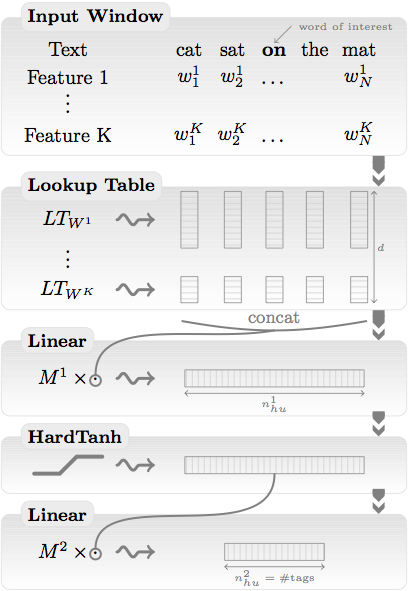
\includegraphics[width=\textwidth]{nnstructure}
  \caption{The basic network structure, using a window
approach. Figure from
\cite[2499]{collobert-2011}.} \label{fig:nnstructure}
\end{figure}

\subsubsection{Lookup table layer} The lookup table itself is a matrix
with $d_{wrd}$ rows and $D$ columns. Its initial construction is as
follows: given a frequency table, the $D$ most common words are chosen
and placed in order. Each word is now assigned an index according to
its ranking in the frequency table. The most common word gets index 1,
the second most common index 2 etc., up to the word in the $D^{th}$
place in the table, which is assigned index $D$. For each index, a new
embedding of size $d_{wrd}$ with small random values is created and
assigned to that index. The lookup table matrix itself is constructed
by concatenating these $D$ vectors as columns.  In this way, a lookup
operation for an index $i$ is actually nothing more than the selection
of the $i^{th}$ column from this matrix.

The lookup table layer itself consists of $wsz$ input neurons; given a
text window, each word is converted to its corresponding index, which
is then fed to the neuron corresponding to its position in the window,
which retrieves the embedding of that word from the lookup table. The
output of all neurons is then concatenated into a single matrix, whose
columns are now the embeddings for the input window.

Formally, given a word index vector $w \in N^{wsz}$ and a lookup table
$L \in R^{d_{wrd} \times D}$, we can express this as as a function
$LT$:

\begin{equation} \label{eq:ltmatrix} LT(L, w) =
\left( \begin{array}{cccc} L_{1,w_1} & L_{1,w_2} & \ldots &
L_{1,w_{wsz}} \\ L_{2,w_1} & L_{2,w_2} & \ldots & L_{2,w_{wsz}} \\
\ldots & \ldots & \ldots & \ldots \\ L_{d_{wrd},w_1} & L_{d_{wrd},w_2}
& \ldots & L_{d_{wrd},w_{wsz}} \end{array} \right)
\end{equation}

An interesting feature of this type of representation is that it is in
fact a highly performant abstraction for the classic $n$-gram. In most
NLP architectures $n$ is given a relatively low value in order to
limit computational expenses; the Google $n$-gram project, which is the
largest of its kind, limits itself to five-grams. N-grams are also
used differently: the first $n - 1$ words serve as the context for the
$n^{th}$ word in the $n$-gram. Here, we can take advantage of the
purely numerical form of text window embeddings by choosing a somewhat
larger text window size and considering the central column in such
windows in its full context, both prior and posterior.

\subsubsection{Linear layer}
A linear layer takes a fixed size vector and performs a linear
operation on it: the dot product of this vector with a set of
parameters $W$ is computed and a bias added. Formally, given the
output vector $f^{l-1}_\theta$ of layer $l-1$, the following
computation is performed in layer $l$:
\begin{equation}
  f^l_\theta = W^l \cdot f^{l-1}_\theta + b^l
\end{equation}
Where $\theta$ indicates the existing parameters of the network and
$W^l \in R^{n^l_{hu} \times n^{l-1}_{hu}} $ and $b^l \in R^{n^l_{hu}} $
are the parameters of the layer to be trained, with $n^l_{hu}$
representing the amount of hidden units in layer $l$. Linear layers
transform their input and several such layers can be stacked, similar
to how linear functions can be composed.

\subsubsection{Hard hyperbolic tangent layer}

If we intend for our network to be able to model a highly nonlinear
system such as language, we need to introduce nonlinearity
somewhere. A good function for this is the hyperbolic tangent, which
is differentiable everywhere and approximates a linear threshold
function very nicely. A layer $l$ using the hyperbolic tangent as an
activation function contains $n^l_{hu}$ neurons taking $n^{l-1}_{hu}$
inputs. In this case, the activation function $g(x)$ for a scalar x
is:
\begin{equation}
  g(x) = tanh(x) = \frac{e^{2x} - 1}{e^{2x} + 1}
\end{equation}
For an input vector generated by a layer $l - 1$, the function $g$ represented by a hyperbolic tangent layer can be defined as:
\begin{equation}
  f^l_{\theta} = g(f^{l-1}_{\theta})
  = \left[ \begin{array}{c}
      g(f^l_{\theta1}) \\
      g(f^l_{\theta2}) \\
      \ldots \\
      g(f^l_{\theta n^{l-1}_{hu}})\\ \end{array} \right]
\end{equation}
We approximate this function using the hard hyperbolic tangent, defined for a scalar as:
\begin{equation}
  hardtanh(x) = = \begin{cases} 1, & \mbox{if } x > 1 \\ -1, & \mbox{if } x < -1 \\ x & \mbox{otherwise.}\end{cases}
\end{equation}
We can define this function for vector inputs in the same manner
as for the hyperbolic tangent function.

\subsubsection{Scoring layer}

The final layer. This is actually simply a linear layer which is
designed to output a vector containing as many elements as there are
possible tags for the task at hand. Each output element is a score
which reflects the probability of the corresponding tag for the
central word in the input window.

\subsection{Unsupervised learning}
\label{sec:unsupervised}

The first phase of learning is unsupervised; large amounts of raw
language data are fed to the network. Instead of training using a
classical squared-loss function, a pairwise ranking function is
introduced. The network is constructed as described in the previous
section; we want a single score $f_{\theta}(x)$ to be output for a
given window of text $x$.  The window is first corrupted using a word
$w$ from the dictionary by replacing the central word in $x$ by
$w$. We express this corrupted window as $x^{(w)}$. The pairwise
ranking of any two such pairs $x$ and $w$ is defined as $r(\theta, x, w) = max\left\{0,
  1 - f_{\theta}(x) + f_{\theta}(x^{(w)})\right\}$. 
In effect, we want the non-corrupted window to achieve a higher score
than the corrupted window. We can achieve this by adjusting the
parameters $\theta$ such that the pairwise ranking of $x$ and $w$ is
minimal, since this implies that $f_{\theta}(x)$ must yield a higher
score than $f_{\theta}(x^{(w)})$. Summing this operation over all
possible pairs $(x, w)$ and defining a mapping from the parameters
$\theta$ to this sum, we obtain a general cost function:
\begin{equation}
  \theta \mapsto \sum\limits_{x \in X} \sum\limits_{w \in D} r(\theta, x, w)
\end{equation}
Where $X$ is the set of possible windows of size $wsz$ and $D$ the chosen
dictionary. Minimizing this function with respect to $\theta$ will
ensure the relevant parameters (the embeddings and the first two
layers) are tuned so that our ranking function $f_{\theta}$ yields
accurate scores. Using this simple criterion, we have a method for
crafting a set of parameters that contains a consistent structured
internal representation of the training data. Despite the relatively
simplicity of the criterion, the huge amounts of parameters results in
a very taxing and lengthy computation. Furthermore, there is no
guarantee that the cost function has a single minimum with respect to
$\theta$; a full grid search would be necessary, which necessitates
vast amounts of computing time. 

% \subsubsection{Curriculum learning}
% \label{sec:curricula}
Instead, the process is sped up using \textbf{curriculum learning};
the basic idea of this technique is analogous to the learning process
children are put through in school: instead of starting their
education with university-level quantities of difficult material
immediately, a restricted set of elementary concepts is introduced on
which they concentrate. Successive phases of learning are performed by
gradually expanding the set of concepts which is to be learned, making
use of earlier concepts to facilitate the understanding of more
complex concepts.

The same method, for reasons not yet fully understood, can be applied
to unsupervised learning.\footnote{Among the scholarship of note on
  this subject we find \citet{bengio2009curriculum} and
  \citet{erhan2010}.} First, the training material is restricted to the
most frequent observations of the process we want to model. Training
over this restricted set creates a simplified model which, due to the
abundance of examples, should be accurate. Subsequently, new
iterations of the learning algorithm are run over successively larger
sets; at each iteration, the model becomes more detailed and describes
more classes of observations more accurately.

This is applied to the problem at hand by choosing
successively larger dictionary sizes. During the calculation of the
minimum of the cost function, windows which are not centered around a
word which is in the dictionary are ignored. This initially entails a
significant reduction of our sets $X$ and $D$, which makes the process
a bit less computationally demanding. Subsequent iterations are
computationally more expensive, but are initialised with the
parameters found by previous iterations; observations previously used
in learning will already return excellent scores and will only
necessitate minor adjustments to the parameters, while new
observations can be fit into the general picture more easily.

% \subsubsection{Genetic model generation}
% \label{sec:geneticmodels}

% The second is genetic model generation by using \textbf{model breeding}. 
% \begin{itemize}
% \item model `breeding'
% \item at each iteration of increasing dictionary sizes, search for
%   optimal parameters
% \item use a validation set: a selection of sentences held out from a
%   corpus
% \item optimise by trying different parameters and then evaluating the
%   accuracy of the network's output for the validation sentences
% \item at each step, pick the best model, then expand on this
%   (`breeding lines')
% \end{itemize}

\subsection{Supervised learning}
\label{sec:supervised}

The supervised training phase involves the creation of task-specific
networks which are initialised with the embeddings created during the
unsupervised phase; these form a shared first part of all networks. A
given network is then tailored to have an adapted output as necessary
for the task of interest. Training proceeds in the classical fashion,
by providing correctly formatted examples and adjusting all parameters
(including the shared ones) to minimize the squared error.

The output of a network of this type is a vector; each specific
feature is encoded in on component of this vector by setting this
component to one and all others to zero. This is called a one-hot
vector. All tasks are jointly trained, that is to say, the networks
share parameters, are trained simultaneously and are allowed to modify
shared parameters. Individual (non-shared) network parameters are
modified only during training for a specific task. This technique
allows us to generalise the training benefit from each example.

Composing such a one-hot vector is not simple for Greek morphology:
any given word will belong to multiple morphological categories. For
instance, a verbal form has a tense, a mood, a number, a person, and
sometimes even a case and gender. Gathering all possible features into a
single one-hot vector is therefore not feasible.

We could approach this problem in different ways. An instinctive test
is to simply feed the system raw parses and assign one component of
the output vector to each possible parse. This is needlessly
complicated; if we look at the list of morphological parses from the
Perseus database, we find more than 2000 distinct morphological
analyses! An output vector of this size is simply too unwieldy.

A more dynamic approach would be to create one-hot vectors for each of
the following categories, with the number of options assigned to each
category corresponding to the number of components in the
corresponding output vector:

\begin{itemize}
\item major part of speech: verb, noun, adjective, pronoun, particle,
  adverb, numeral, preposition, conjunction, interjection;
\item minor part of speech: article / determinative, personal,
  demonstrative, indefinite, interrogative, relative, possessive,
  reflexive, reciprocal, proper;
\item person: first, second, third;
\item number: singular, plural, dual;
\item tense: present, imperfect, aorist, perfect, pluperfect,
  future, future perfect;
\item mood: indicative, subjunctive, optative, imperative,
  infinitive, participle, gerundive, gerund, supine;
\item voice: active, middle, passive, middle-passive;
\item gender: masculine, feminine, neuter, common;
\item case: nominative, genitive, dative, accusative, ablative,
  vocative;
\item degree: comparative, superlative.
\end{itemize}

\begin{table}
  \begin{tabular}{|l|l|l|}
    \hline
    \textbf{field}            & \textbf{category} & \textbf{possible values} \\ \thickhline
    first field  & lemma type & \specialcell{a - adjective\\c - conjunction\\d - adverb\\e - exclamation\\g - particle\\l - article\\m - numerals\\n - noun\\p - pronoun\\r - preposition\\t - participle\\v - verb\\x - miscellanea} \\ \hline
    second field & person & \specialcell{1 - first person\\2 - second person\\3 - third person} \\ \hline
    third field  & number & \specialcell{d - dual\\p - plural\\s - singular} \\ \hline
    fourth field & tense & \specialcell{a - aorist\\f - future\\i - imperfect\\l - pluperfect\\p - present\\r - perfect\\t - future perfect} \\ \hline
    fifth field & mood & \specialcell{g - gerund \\ p - participle \\ i - indicative\\m - imperative\\n - infinitive\\o - optative\\s - subjunctive} \\ \hline
    sixth field & diathesis & \specialcell{a - active\\e - energetic\\m - medial\\p - passive} \\ \hline
    seventh field & gender & \specialcell{f - feminine\\m - masculine\\n - neuter\\ o, p and q - unclear} \\ \hline
    eighth field & case & \specialcell{a - accusative\\d - dative\\g - genitive\\n - nominative\\v - vocative} \\ \hline
    ninth field & degree of comparison & \specialcell{c - comparative\\s - superlative} \\ \hline
    \hline
  \end{tabular}
  \caption{The Perseus ennealiteral morphological abbreviation system.} \label{table:perseusmorph}
\end{table}

\begin{table}
  \begin{tabular}{|l|l|l|}
    \hline
    \textbf{field}            & \textbf{category} & \textbf{possible values} \\ \thickhline
    first field & person & \specialcell{1 - first person\\2 - second person\\3 - third person} \\ \hline
    second field  & number & \specialcell{d - dual\\p - plural\\s - singular} \\ \hline
    third field & tense & \specialcell{a - aorist\\f - future\\i - imperfect\\l - pluperfect\\p - present\\r - perfect\\t - future perfect} \\ \hline
    fourth field & mood & \specialcell{i - indicative\\m - imperative\\n - infinitive\\o - optative\\s - subjunctive} \\ \hline
    fifth field & diathesis & \specialcell{a - active\\e - energetic\\m - medial\\p - passive} \\ \hline
    sixth field & gender & \specialcell{f - feminine\\m - masculine\\n - neuter} \\ \hline
    seventh field & case & \specialcell{a - accusative\\d - dative\\g - genitive\\n - nominative\\v - vocative} \\ \hline
    eighth field & degree of comparison & \specialcell{c - comparative\\s - superlative} \\ \hline
    ninth field & placeholder column & \specialcell{-} \\ \hline
    tenth field & inflectibility & \specialcell{i - inflected\\n - not inflected} \\ \hline
    \hline
  \end{tabular}
  \caption{The PROIEL decaliteral morphological abbreviation system.} \label{table:proielmorph}
\end{table}

\begin{table}
  \begin{tabular}{|l|l|l|}
    \hline
    \textbf{field}            & \textbf{value} & \textbf{Perseus first field equivalent} \\ \thickhline
    A- & adjective & $\rightarrow$ a \\ \hline
    C- & paratactic conjunctions & $\rightarrow$ c \\ \hline
    Df & adverbs & $\rightarrow$ d \\
    Dq & adverbial response particles (where, how, etc.) & $\rightarrow$ g \\
    Du & adverbial question particles (where, how, etc.)  & $\rightarrow$ g \\ \hline
    F- & Hebrew loan words & $\rightarrow$ x \\ \hline
    G- & hypotactic conjunctions & $\rightarrow$ c \\ \hline
    I- & illocutive particles & $\rightarrow$ g \\ \hline
    Ma & cardinal numerals & $\rightarrow$ m \\
    Mo & ordinal numerals & $\rightarrow$ m \\ \hline
    Nb & nouns (in general) & $\rightarrow$ n \\
    Ne & nouns (proper names) & $\rightarrow$ n \\ \hline
    Pc & pronouns (reciprocative) & $\rightarrow$ p \\
    Pd & pronouns (demonstrative) & $\rightarrow$ p \\
    Pi & pronouns (interrogative) & $\rightarrow$ p \\
    Pk & pronouns (reflexive) & $\rightarrow$ p \\
    Pp & pronouns (personal) & $\rightarrow$ p \\
    Pr & pronouns (relative) & $\rightarrow$ p \\
    Ps & pronouns (possessive) & $\rightarrow$ p \\
    Px & pronouns (quantitative, i.e.\ some, all, none, same, other) & $\rightarrow$ x \\ \hline
    R- & prepositions & $\rightarrow$ r \\ \hline
    S- & article & $\rightarrow$ l \\ \hline
    V- & verb & $\rightarrow$ v \\ \hline
    \hline
  \end{tabular}
  \caption{The PROIEL biliteral lemmatic abbreviation system.} \label{table:proiellemmata}
\end{table}

\begin{table}
  \begin{tabular}{|l|l|}
    \hline
    \textbf{The Perseus system} & \textbf{The PROIEL system} \\ \thickhline
    \begin{minipage}{2.5in}
      \begin{itemize}[noitemsep,topsep=0pt,parsep=0pt,partopsep=0pt]
      \item adv: adverbial;
      \item apos: apposing element;
      \item atr: attributive;
      \item atv/atvv: complement;
      \item auxc: conjunction;
      \item auxg: bracketing punctuation;
      \item auxk: terminal punctuation;
      \item auxp: preposition;
      \item auxv: auxiliary verb;
      \item auxx: commas;
      \item auxy: sentence adverbials;
      \item auxz: emphasizing particles;
      \item coord: coordinator;
      \item exd: ellipsis;
      \item obj: object;
      \item ocomp object complement;
      \item pnom: predicate nominal;
      \item pred: predicate;
      \item sbj: subject.
      \end{itemize}
    \end{minipage} &
    \begin{minipage}{2.5in}
      \begin{itemize}[noitemsep,topsep=0pt,parsep=0pt,partopsep=0pt]
      \item adnom: adnominal;
      \item adv: adverbial;
      \item ag: agens;
      \item apos: apposition;
      \item arg: argument (object or oblique);
      \item atr: attribute;
      \item aux: auxiliary;
      \item comp: complement;
      \item expl: expletive;
      \item narg: adnominal argument;
      \item nonsub: non-subject (object, oblique or adverbial);
      \item obj: object;
      \item obl: oblique;
      \item parpred: parenthetical predication;
      \item part: partitive;
      \item per: peripheral (oblique or adverbial);
      \item pid: Predicate identity;
      \item pred: predicate;
      \item rel: apposition or attribute;
      \item sub: subject;
      \item voc: vocative;
      \item xadv: open adverbial complement;
      \item xobj: open objective complement;
      \item xsub: external subject.
      \end{itemize}
    \end{minipage} \\ \hline
  \end{tabular}
  \caption{The Perseus and PROIEL syntactic annotation systems.} \label{table:proielmorph}
\end{table}

This approach has its downside: we now have to train distinct networks
for each network. The upside, though, is that each of these networks
is much, much smaller than a single network mapping all possible
parses and will be easier to train; an example of the
divide-and-conquer technique. We could possibly be confronted with
impossible parses, such as an 'imperfect optative', but this is highly
unlikely due to the total absence of examples for this form.

The task of preprocessing the corpus, which is discussed
\textit{infra}, is also simplified due to this approach: the two main
corpora from which the training material is gathered use similar but
slightly different annotation schemes. The PROIEL system is a bit more
complex, but essentially gives the same information as the Perseus
system. Tables 1 and 2 offer a detailed overview of both systems;
table 3 contains conversion guidelines. For simplicity's sake, we pick
the Perseus system, since this limits the amount of networks we'd have
to train to nine. Instead of having to convert from one type of
annotation to another, we can simply split the annotations into their
constituent parts, store them in different files and resolve any
annotational differences afterwards with minimal headaches.

The process of dependency annotation only requires one network, but is
a bit more complex. The source corpora for the training data once
again use similar annotation schemes but with different emphases. We
enumerate the tags for the Perseus and the PROIEL annotation system,
respectively.

We see in table 4 that they respectively use nineteen and twenty-four
different features. The Perseus system is less detailed than the
PROIEL system, but by virtue of this fact also less complex. A
possible approach is to map overlaps in both systems and find the
simplest possible tag set which can be derived from that. We can
immediately make a one-hot vector from this, since all annotated words
are equipped with a single syntactic tag. 

Another approach is provided in \cite{conf/lrec/LeeH10}, who attempt
to port the Perseus treebank to the PROIEL format. The approach has
its downside: the authors try to convert every detail of the Perseus
treebank format to the PROIEL format and achieve an accuracy rate
which still necessitates human postprocessing. We will consider it
feasible to switch to their system once a full-fledged conversion from
one scheme to the other has been carried through to completion. Until
then, we apply a simpler system with reduced information
density. Since we do not have to cope with head-dependency relations,
we use the simpler approach to reduce computational overhead in our
experimental setup.

\section{Selecting and processing training data}
\label{sec:trainingdata}

For the unsupervised learning phase, we need a maximally large
corpus. I chose the TLG CD-ROM E, which contains about 9.3M words, and
the Perseus texts, which contain about 7.7M words. Since both corpora
shared material, duplicated sentences were scrapped. The final corpus
contains about 16.9M words. For training the model, this corpus is
split sentence-wise into a training corpus, from which representations
are learned, and a validation corpus, to check the accuracy of the
generated representations. The file is split 90-10.

The supervised learning phase makes use of the Perseus treebank and
the PROIEL annotated texts of Herodotus and the New Testament. These
respectively contain approx. 350K and 195K words, making for a total
of about 545K words. Again, a validation set is withheld, in a
slightly lower proportion than in the unsupervised phase due to the
restricted size of the corpus.

All texts are preprocessed by converting all words to lowercase and
placing exactly one sentence on every line. Only Greek punctuation is
left; critical notation etc. is pruned.

\section{Annotating the corpus}
\label{sec:annotating}

After the architecture (model and networks) is built, it is
serialised; that is to say, the internal state of the architecture
during training time is stored to disk. Serialisation allows us to
immediately load the model into memory during the execution of our
tagging program. When tagging, we use the architecture in a read-only
manner, i.e. we only predict and do not adjust parameters any more.

Tagging is essentially a process of probabilistic prediction; text
windows are passed through each of the networks, which return a
prediction of the expected features of the central words in these
windows in the form of an output vector. For tagging a sentence with
$n$ words, we create $n$ text windows and use these as input. Each
window generates an output vector; we pick the component with the
maximum score and attribute the corresponding tag to the central word
in the original text window. This process is iterated over every
sentence in the target text. 

% In order to find the most likely sequence of tags, we can use the
% Viterbi algorithm. Suppose we have a matrix $A \in R^{m \cross n}$. We
% can convert this matrix to a graph G by associating every component of
% the matrix to an edge and a node and adding $m$ nodes which correspond
% to a start state $q_0$. 
% \begin{itemize}
% \item find the most likely sequence using Viterbi decoding
% \item when viewing the matrix as a graph, we can trace a path through
%   this matrix
% \item edge weights are probabilities of any tag following another
%   given a word following another
% \item nodes are states, that is, word-tag correspondences
% \item the path with the largest product of edge weights corresponds to
%   the most likely tag sequence
% \end{itemize}

%************************************************
\chapter{Implementation}
\label{chp:implementation}
%\minitoc\mtcskip
%************************************************

\section{Language and source code}
\label{sec:langsource}
\subsection{Choice of language}
\label{sec:language}

\begin{itemize}
\item Python
\item concise and simple syntax
\item slow language, fast numerical libraries: Numpy, Scipy, Theano, Matplotlib ...
\item excellent Unicode support since version 3
\end{itemize}

\subsection{Source code availability}
\label{sec:sourcecode}

\begin{itemize}
\item GitHub
\item based off J. Turian's implementation but documented, cleaned up, improved ...
\end{itemize}

\section{The full process}
\label{sec:process}

\subsection{Preparing the training corpora}
\label{sec:trainingcorpora}
\begin{itemize}
\item conversion from TLG or TEI format to raw text
\item conversion from Beta Code to Unicode
\item stripping all characters which are not relevant, such as
critical notation, paragraph markers etc.
\item lowercase all words
\item detailed tokenisation is not necessary
\item convert annotation to a unified system
\item create conversion script from classic annotation to one-hot vector annotation
\end{itemize}

\subsection{Training the model}
\label{sec:createmodel}
\begin{itemize}
\item window size of 11 words, due to the frequency of long-range dependencies in Greek
\item represent features in 50-dimensional vectors (more dimensions
  could affect the computation time adversely)
\item unsupervised iterations over increasing dictionaries: 5.000,
10.000, 20.000, 40.000, 80.000, 160.000, 360.000
\item stop at the point of diminishing returns (computing the ranking
for a dictionary of 360.000 given a corpus of size n requires 360.000
ranking formula calculations, which is bound to take a lot of time)
\item continue training, now supervised but with the same hyperparameters and parameters as the supervised model
\end{itemize}

\subsection{Preparing the object corpus}
\label{sec:createmodel}
\begin{itemize}
\item conversion from  TEI format to raw text
\item one sentence per line!
\item stripping all characters which are not relevant, such as
critical notation, paragraph markers etc. but padding the text where necessary
\item store tags sequentially
\item basic tokenisation is handled during tagging
\item run sentence through networks, then concatenate relevant outputs
\item convert from one-hot vector notation to classic annotation
\item iterate over every sentence
\item done!
\end{itemize}

\part{Results \& discussion}
\label{part:results}
%************************************************
\chapter{Results}
\label{chp:results}
%\minitoc\mtcskip
%************************************************

\section{Experimental setup}
\label{sec:computationtime}

\subsection{Training material}
\label{sec:trainingmaterial}
For the unsupervised learning phase, we need a maximally large
corpus. We chose the TLG CD-ROM E, which contains about 9.3M words, and
the Perseus texts, which contain about 7.7M words. Since both corpora
share material, duplicate sentences were scrapped. The final corpus
contains about 16.9M words.

This corpus was split sentence-wise into a training corpus, from which
representations are learned, and a validation corpus, to check the
accuracy of the generated representations. The file is split 90-10.

The supervised learning phase makes use of the PROIEL annotated texts
of Herodotus and the New Testament for both morphology and
syntax. This contains approx. 195K words. Again, a validation set is
withheld, in a slightly lower proportion than in the unsupervised
phase due to the restricted size of the corpus.

\subsection{Execution}
\label{sec:execution}

Corpus preprocessing was done on the author's own computer. We then
conducted training on an Amazon EC2 compute-optimized instance. The
unsupervised algorithm was left to generate embeddings for *FILL IN
TIME* hours.  This was equivalent to *FILL IN EPOCHS* training
epochs. The supervised algorithm was left to iterate over the
annotated corpus, finishing in *FILL IN HOURS*. Logs of the training
process was generated and can be found in appendix
\vref{chp:traininglog}. We then tagged the correctly aligned corpus
using the generated model, which took *FILL IN HOURS*.

\subsection{Output format}
\label{sec:output}

The resulting language model was then serialised for immediate reuse;
a dump of the model parameters was also created in HDF5 format. The
tagged corpus was converted from plain text to the CoNLL markup scheme
and to TEI-compliant XML.

\section{Performance}
\label{sec:performance}

\subsection{Unsupervised model}
\label{sec:unsupacc}

To quickly get a general picture of the quality of the embeddings, we
pick ten words throughout the lookup table and take their ten nearest
neighbors in the vector space according to the Euclidean metric. *TABLE REFERENCE*

We then validate the model by computing rankings for each word using a
simple heuristic: we generate text windows from the validation corpus,
to which we let the model assign a score. For each window, we generate
a score for each possible corrupted version of the window (i.e. we
replace the central word index by all other word indexes
iteratively). The ranking of the word corresponds to the amount of
corrupt windows which receive a higher score than the original
window. We then compute the mean and standard deviation of the
logarithms of these rankings. *TABLE REFERENCE*

\subsection{Supervised model}
\label{sec:supacc}
For the supervised model, we use a more straightforward approach: we
strip the validation corpus of annotation and tag it using the
model. We then compare the original annotation with the newly
generated annotation and note the accuracy percentage. *TABLE REFERENCE*

\subsection{Goal corpus}
\label{sec:supacc}
For the goal corpus, we may only evalute the accuracy of the
embeddings. We use the same method as for the validation set for model
training. *TABLE REFERENCE*
%************************************************
\chapter{Assessment \& conclusion}
\label{chp:assessment}
%\minitoc\mtcskip
%************************************************

\section{Evaluation \& Hypothesis}

\subsection{Unsupervised model}
\subsection[Unsupervised model]{Unsupervised model\footnote{We did not have time to compute word rankings. We did pick a few words to test the rankings, but they were not good (generally in the upper part of the spectrum for rankings).}}
For unsupervised training, we attained reasonable results as shown in the
figures in the previous section. For the first few curricula, scoring
accuracy during training steadily increased, but then decreased during
the last curriculum, using the full vocabulary. This is due to the
fact that this last curriculum contained 300K more words than the
penultimate one, all of which needed to be trained. We also integrated
sentence padding during this last curriculum, which increases the
amount of words to be processed by a large margin.

The progress of training might seem discouraging, but it is good to
keep in mind that the average score of a correct window is a good deal
higher than that of a corrupted window, and that in general the model
evolves positively until the addition of the last curriculum, which is
of relatively little importance at this stage because of the rarity of
the words it adds.

We only computed select word rankings and were confronted with the
fact that most of them were not good. We propose that the trainer
needs much more time.

\subsection{Supervised model}
The supervised model is most certainly the weakest part of our
architecture. For the sake of simplicity, we did not implement any
safeguards for our morphological analyses, and now pay for it: the
system assigns tags without too much regard for the rules of Greek
grammar. For instance, for the first sentence of our test corpus, not
a single tag is correct. Nouns are assigned tenses, moods, etc ... It
is evident that we have not even approached the accuracy rates of
\cite{mambrini2012} and \cite{dik2008,dik2009}. We believe this is in
part also due to the relatively small training corpus for the
supervised phase.


% What are the major patterns in the observations? (Refer to spatial and temporal variations.)
% What are the relationships, trends and generalizations among the results?
% What are the exceptions to these patterns or generalizations?
% What are the likely causes (mechanisms) underlying these patterns resulting predictions?
% Is there agreement or disagreement with previous work?
% Interpret results in terms of background laid out in the introduction - what is the relationship of the present results to the original question?
% What is the implication of the present results for other unanswered questions in earth sciences, ecology, environmental policy, etc....?
% Multiple hypotheses: There are usually several possible explanations for results. Be careful to consider all of these rather than simply pushing your favorite one. If you can eliminate all but one, that is great, but often that is not possible with the data in hand. In that case you should give even treatment to the remaining possibilities, and try to indicate ways in which future work may lead to their discrimination.


\section{Concluding remarks}
\label{sec:conclusion}
We have given a brief but complete \textit{status quaestionis} of the
scholarship on NLP for ancient Greek, something which we did not find
anywhere else. We consider that we have a made a modest methodological
contribution by attempting to use techniques which as of yet have not
been applied to ancient Greek, even though the results are
disappointing. Furthermore, the unsupervised technique shows promise
if given more time to train. We offer some perspectives on how our
work should be improved and continued.

\section{Further work}
\label{sec:further_work}
\subsection{Improving the language model}
\subsubsection{Larger training sets}
Improving the unsupervised model can be done in two ways: by running
the unsupervised modeling phase for more epochs, or by increasing the
amount of training data. The first option is certainly feasible at
this point, but our training set exhausts most of the available
material. 

A first option is the corpus of papyri; however, we chose to exclude
it from the training set to avoid skewing the results. But the most
obvious option is the integral \textit{Thesaurus Linguae Graecae},
which contains more than 109M words but is still not freely
available. This is an order of magnitude larger than our current
training corpus! This is a huge amount of resources which we can
exploit to improve our model.

The main reason for these texts not being published in a downloadable
format is that the TLG requires funds to run its servers. However, we
still find it hard to justify that such a rich resource for classical
scholarship should not be distributed more widely to facilitate
further study. While this is no place for an extended philippic in
favour of open-sourcing the TLG, we still think a strong case can be
presented for this.

The supervised component of our model can also be improved by running
more epochs (which we did not have time for), but especially by
increasing the size of the training corpus. We opted to only use the
PROIEL treebank and not the Perseus treebank to minimise headaches
related to the conversion of one annotation standard to
another. Especially the syntactic annotation standards used by both,
while sharing some common concepts, are very different in
implementation.

This could be fixed by developing an effective and accurate system for
this type of conversion; this has been attempted in
\cite{conf/lrec/LeeH10}, but the accuracy rate of that experiment (in
the low 80\%s for both Latin and Greek) is too low to allow extended
use. In any case, it is our opinion that developing a more unified
system for ancient Greek treebanks is a \textit{desideratum} before
the scale of current treebanks is expanded, lest we end up with two
competing standards with none of both to lead us into the fray.

\subsubsection{Linguistic foreknowledge}
We chose our training method because of its simplicity; but it is a
good question whether it is possible to use more linguistic
foreknowledge strategically. \cite{collobert-2011} equip their model
with a selective set of simple linguistic features which are tuned to
improve performance for certain tasks. For instance, they improve
performance for named entity recognition by adding a feature for
capitalisation, which is handy given the use of capital letters in
English to indicate proper nouns. They also equip their system with a
gazetteer, which is a large list of proper nouns.

Similarly, we could recruit supplemental resources to improve
performance at our chosen tasks as well as others \ref{sec:expand}. A
large database of morphological parses exists in the form of the SQL
dump of the Perseus word study tool. We could implement a supplemental
network which reduces the number of possible parses for each word
which is in this database and is trained to pick the correct one; if
it is not, we use the unmodified neural architecture to estimate a
likely parse.

A similar technique we could use is cascading. Using this technique,
we train taggers for diverse tasks which are interconnected; we apply
these taggers sequentially and use the outputs of previous taggers for
each task. In this way, we can also heavily limit possibilities. For
example, by first finding the correct part-of-speech for a word, we
can immediately eliminate certain morphological categories. A noun,
for instance, has no voice, tense or mood, and developing such
sequential tagging method would prevent us from spending valuable
computation time on these 'no-brainers'.

\subsubsection{Probabilistic parameters}
Our model as it stands is actually very simple, a card which we have
unsuccessfully tried to play out against the complexity of Greek. We
therefore propose to add extra parameters to the model. More
specifically, we would like to add supplemental parameters for
probabilistic inference on two levels: the level of morphological
parsing and the level of sentence structure. As it stands, we compute
probabilities of tags being correct for individual word windows, but
the main weakness in this approach is that we do not check either the
consistency of morphological parses or the likelihood of a given tag
sequence.

This could be remedied by developing transition tables for each
distinct problem and applying these during tagging. During training,
counts of tag transitions would be kept inside these tables and
involved in training the parameters. This is an approach also proposed
by \cite{collobert-2011} which we have not implemented due to a lack
of time. In this way, we could ensure that our tags are not as
nonsensical as they have in our experiment.

\subsubsection{Expansion and integration}
A key point for the further development of a large-scale
infrastructure for ancient Greek annotated corpora is the integration
of diverse resources. We find an example of this in the recent
merger of several papyrological resources on the web into
\texttt{papyri.info}. The recently announced Open Philology Project
\citep{crane2013} is another good example of this kind of enterprise.

We propose the development of a full NLP stack for corpus
annotation. We envision this as a library similar to the Python
Natural Language Toolkit \citep{nltkhome}, which will offer a diverse
range of tools tailored for ancient Greek: tokenizers, POS taggers,
chunkers, parsers, training tools, concordance creators ... This tool
could then be integrated with other digital classics resources.

\subsubsection{Expanding the range of tasks}
\label{sec:expand}
Another interesting prospect is the expansion of the architecture to a
larger array of tasks. The possibilities, are certainly there:
\cite{collobert-2011} explores named entity recognition
(\textit{cfr.supra}) and semantic role labeling with noteworthy
success. Deep parsing using the same type of embeddings with recurrent
neural networks has shown excellent results, as shown in
\cite{collobert2011deep}, which attains benchmark performance. 

All of this is done using large-scale unsupervised learning with a
small kernel of supervised training data, the same technique we have
applied. The same method would also fit for ancient Greek; but again
progress is blocked by a lack of annotated language data. 

% \section{Named entity recognition}
% \label{sec:ner}

% Named entity recognition is a subdiscipline in natural language
% processing which is concerned with the automatic extraction and
% localisation of all kinds of names from texts. It has been used
% extensively in literary texts with a view to discern the importance of
% certain characters throughout the text. The KU Leuven's long-standing
% Prosopographia Ptolemaica project, which aims to be a repository of
% all inhabitants of Egypt between 300 and 30 B.C., could easily benefit
% from these techniques. The abundant manual labour that has gone into
% the project could be fed as training data to and then supplemented by
% a named entity recognition engine that could also categorise personal
% names by any criteria and establish contextual relations between
% them. To take a very rudimentary example, the name 'Alexander' could
% be retrieved in all texts and a cluster of related names generated, so
% that related individuals may be placed in a web of relations; or one
% could ask, by combining the already present linguistic annotation, to
% display all adjectives which accompany the name 'Alexander'.

% It could even go further than this and also include other particular
% names, such as places, distances, monetary units, weights, and so
% on. Historians could create a comprehensive overview of, for instance,
% the inflation of Egyptian currency, or map out trade connections using
% a search for all mentions of currency, weight and places which are in
% proximity to each other.



% What are the things we now know or understand that we didn't know or understand before the present work?
% Include the evidence or line of reasoning supporting each interpretation.
% What is the significance of the present results: why should we care? 
% % **************************************
\chapter{Further work} % (fold)
\label{cha:further_work} % **************************************


\section{Improving the language model}
\subsection{Larger training sets}
\begin{itemize}
\item mainly: TLG holds much more text but does not free it
\item connection with projects like Open Philology: build large tagged
corpora using crowdsourcing
\end{itemize}
\subsection{Linguistic foreknowledge}
\begin{itemize}
\item simplicity is strength of model
\item can we use foreknowledge strategically?
\end{itemize}
\subsection{Expanding the range of tasks}
\subsubsection{Stemming}
\subsubsection{Named entity recognition}
\subsubsection{Semantic role labeling}
\subsubsection{Deep parsing}
% \section{Named entity recognition}
% \label{sec:ner}

% Named entity recognition is a subdiscipline in natural language
% processing which is concerned with the automatic extraction and
% localisation of all kinds of names from texts. It has been used
% extensively in literary texts with a view to discern the importance of
% certain characters throughout the text. The KU Leuven's long-standing
% Prosopographia Ptolemaica project, which aims to be a repository of
% all inhabitants of Egypt between 300 and 30 B.C., could easily benefit
% from these techniques. The abundant manual labour that has gone into
% the project could be fed as training data to and then supplemented by
% a named entity recognition engine that could also categorise personal
% names by any criteria and establish contextual relations between
% them. To take a very rudimentary example, the name 'Alexander' could
% be retrieved in all texts and a cluster of related names generated, so
% that related individuals may be placed in a web of relations; or one
% could ask, by combining the already present linguistic annotation, to
% display all adjectives which accompany the name 'Alexander'.

% It could even go further than this and also include other particular
% names, such as places, distances, monetary units, weights, and so
% on. Historians could create a comprehensive overview of, for instance,
% the inflation of Egyptian currency, or map out trade connections using
% a search for all mentions of currency, weight and places which are in
% proximity to each other.

\section{Refining the corpus}
\label{sec:refiningcorpus}

\subsection{Collaborative editing}
\label{sec:collaborative}
% The IDP project is heading into crowdsourcing territory at full steam,
% and excluding our own work from this movement would be inserting a
% shrill note into this symphony. All data is placed on GitHub at
% \url{https://github.com/sinopeus/tjufy}, freely accessible and
% editable for all.

% This opens promising avenues of inquiry that do not have a direct
% relation to this thesis. For instance, it can in the future be
% integrated into SoSOL and absorbed into the larger codebase for the
% IDP project if it does not create too much overhead for the current
% developers (the technical back end of the IDP seems to be labyrinthine
% and adding new layers of complexity might be off-putting). It could
% even grow into a separate project which itself could be linked to
% \texttt{papyri.info} as the HGV, APIS and Trismegistos currently are,
% by a common system of indexation.

% Making the code publically available to all also has the advantage of
% the public eye inspecting the texts; using solely automatic analysis
% is bound to deliver an inaccurate result, however small that
% inaccuracy may be, as creating a NLP engine perfectly capable of
% understanding language would be the equivalent of creating a perfect
% artificial intelligence. Therefore, considering the size of the
% corpus, one must rely upon the intelligence of the community. In the
% same way open source software backed by large communities is often of
% excellent quality due to public inspection, the potential for a
% crowdsourced corpus is immense.

\subsection{Linking with other resources}
\label{sec:linking}

\subsubsection{D. Bamman}
\cite{bammanpbml2008,bammantlt8,bammancrane2011}

\subsubsection{The Open Philology Project}
\begin{itemize}
\item possible to integrate papyri?
\item also uses automated approaches
\end{itemize}


% \chapter{Conclusion} % (fold)
\label{cha:conclusion}

% chapter Conclusion (end)



% *****************************************************************
% back matter
%******************************************************************
\backmatter
\clearpage
%*******************************************************
% Bibliography
%*******************************************************
\nocite{*}
\printbibliography


\clearpage
% %************************************************
% \appendix
% \chapter{Appendix}
% \label{chap:appendix}
% %************************************************
\appendix
\pretocmd{\chapter}{%
  \clearpage
  \pagenumbering{arabic}%
  \renewcommand*{\thepage}{\thechapter-\arabic{page}}%
}{}{}

\chapter{Concepts and techniques}
\label{chp:conceptstechniques}
\section{Mathematics}
\label{sec:mathematics}


\subsection{Set theory}
\label{sec:settheory}

Consider an object $o$ and a set $A$. We write 'object $o$ is an
element of set $A$' as $o \in A$. Sets themselves are also objects and
can belong to other sets. Consider two sets, $A$ and $B$. We write
that $A$ is a subset $B$ as $A \subseteq B$; this implies that $B$
contains all elements in $A$ and does not exclude the possibility of
$A$ = $B$; if $A$ is a proper subset of $B$, i.e. all elements of $A$
are in $B$ but not all elements of $B$ are in $A$, we write $A \subset
B$. Mirroring these symbols from right to left gives us the symbols
for supersets and strict supersets, respectively. The empty set, which
contains no elements, is written as $\varnothing$.

There exist different binary operators on sets (i.e. operators on two
sets) which return another set. The most common operators are:
\begin{itemize}
\item the union of sets, written as $A \cap B$, denotes a set which
  contains all elements which are in $A$ and $B$;
\item the intersection of sets, written as $A \cup B$, denotes a set
  which contains all elements which are in both $A$ and $B$;
\item the difference of sets, written as $A \setminus B$, denotes a
  set which contains every element from $A$ excluding those which are
  also in $B$.
\item the Cartesian product of sets, written as $A \times B$, is the
  set containing all ordered pairs of elements from $A$ and $B$.
\end{itemize}

\subsection{Probability}
\label{sec:probability}

A \textbf{probability} is a measure for the likelihood of an event for an
experiment, which we intuitively understand to be an action whose
outcome we want to observe. Such events are then elements of a set
containing all possible outcomes of an experiment; an event can be a
point or subset of that set. We call this set the \textbf{sample space},
denoted S. We denote the probability of an event E as P(E).

Axiomatically, we can define probability as follows:

\begin{enumerate}
\item For every event $E$, $P(E) \geq 0$; no event can have a negative probability.
\item $P(S) = 1$; that is to say, every experiment has an event.
\item For any sequence of disjoint events $A_i$ (that is to say,
  there is no overlap between events), the probability of any one of
  these events occurring is the sum of their respective probabilities.
\end{enumerate}

A few other important properties of probabilities and events are the following:

\begin{enumerate}
\item The complement of an event $A$, which is the union of all
  elements of $S$ which are not an element of $A$, is denoted $A^C$;
  $P(A^C)$ is the probability of this event occurring and is equal to $1
  - P(A)$.
\item For any event E, $0 \leq P(E) \leq 1$.
\item Given any two events $A$ and $B$, $A \subset B \rightarrow P(A) \leq P(B)$.
\end{enumerate}

Given probabilities of a number of events, we can establish
relationships between these probabilities and compute related
probabilities using certain rules. A classic rule is the
\textbf{multiplication rule}, which states that if we perform an
experiment in $k$ parts and the $i^{th}$ part of the experiment has
$n_i$ possible outcomes, and the outcomes of prior parts of the
experiment do not affect latter ones, the probability of any specific
sequence of partial outcome will be the product of all outcome counts
$n_i$ with $i$ ranging from $1$ to $k$.

Set theory is important when we want to know the probability of an
event E which can be constructed from a set of sets $A_i$ using set
operators. The third axiom of probability has already given us the
solution for disjoint events; events may also overlap, and in this
case, we need a more sophisticated formula. For the union of any $n$
events $A_i$, the following holds:
\begin{equation}
  P(\bigcup_{i=1}^n A_i) = \sum\limits_{i=1}^n P(A_i)
\end{equation}

For the intersection of these $n$ events $A_i$, it can be proven that:
\begin{equation}
  P(\bigcap_{i=1}^n A_i) = \lim_{n \to \infty} P(A_i)
\end{equation}
Knowing both these rules is important when considering
\textbf{conditional probability}; for two events $A$ and $B$, suppose
we know $B$ has occurred and we want to know what the probability of
$A$ occurring is given this information. We call this the conditional
probability of $A$ given $B$ and write it $P(A|B)$. If $P(B) > 0$,
then we define it as:

\begin{equation}
  P(A|B) = \frac{P(A \cap B)}{P(B)}
\end{equation}

Using this formula, we can directly derive \textbf{Bayes' theorem} as follows:

\begin{equation}
  \begin{aligned}
    P(A|B) &= \frac{P(A \cap B)}{P(B)} \\
    P(A|B) P(B) &= P(A \cap B)\\
    P(A|B) P(B) &= P(B \cap A)\\
    P(A|B) P(B) &= P(B|A) P(A)\\
    P(B|A) &= \frac{P(A|B) P(B)}{P(A)}
  \end{aligned}
\end{equation}

\subsection{Calculus and linear algebra}
\label{sec:calculus}

\subsubsection{Derivates and extrema}
The derivative of a function is a measure of its rate of change. For a
function in one variable, we can visualise the derivative as a
function which for each point gives the slope of the tangent line to
the original function. Derivatives can be used to find the extrema of
a function, that is to say, the 'low' and 'high' points, with the help
of the fact that the tangent line at these extrema has slope zero. By
'following' the direction indicated by the derivative, we can find
such extrema.

Derivatives are defined for functions with any number of variables,
and so are extrema. The derivative of a multivariable function is
called a gradient; this is a vector with each component containing the
partial derivative of the function with respect to a single of its
variables. We can find extrema for multivariable function by applying
the same method as we do for functions in one variable, by 'following'
the gradient. This is called gradient descent or ascent, depending on
whether we want to find a minimum or a maximum for a function.

\subsection{Statistics}
\label{sec:statistics}
    \subsubsection{Regression}

    Regression is a classic technique from statistics, often visualised as
    'fitting a line to a set of points'. Classification is a related
    technique which uses regression to classify new data points. This is
    essentially what any probabilistic model for natural language
    processing does, in one form or another. What follows is an overview
    of various types of regression and corresponding methods for
    classification.

    We start with \textbf{univariate linear regression}. Given a set
    of $n$ points in the plane, we want to find a hypothesis that best
    corresponds to the location of these points, and we want this
    hypothesis to be a linear function. This function is then of the form:
    \begin{equation}
      h_w(x) = w_1x + w_0
    \end{equation}
    Unless all points are collinear, it is of course impossible to
    find a function of this form that gives a correct mapping for each
    point. The best we can do is find the values of $w_o$ and $w_1$ for
    which the empirical loss on the mappings is minimal. The traditional
    way of doing this is to define a function that computes the squares of
    the errors and sums it over all data points; this is called an
    \textbf{$L_2$ loss function}. We now want to find the values of $w_0$
    and $w_1$ for which this function attains a minimum. We can find these
    minimal points by solving for the roots of the partial derivative
    functions of this loss function with respect to $w_0$ and $w_1$.  This
    problem is mathematically relatively simple and has a unique
    solution. This solution is valid for all loss functions of this type.

    Problems arise when we are trying to create a nonlinear model. In
    this case, the minimum loss equations frequently do not have a unique
    solution. We can of course still model the problem algebraically, and
    the goal is the same: finding the roots of the partial derivative
    function. Now, however, we need to use a more sophisticated method:
    \textbf{gradient descent}. We can visualise this technique as
    'descending a hill'; the 'hill' is the graphical representation of the
    root of the system of partial derivatives, and by 'descending' this
    hill, i.e. by iteratively picking values which bring us closer to the
    bottom part of the valley next to the hill, which corresponds to the
    minimal point of the function, eventually convergence will be reached
    on the minimum and we will found the correct weights for our
    function. The difference by which we change the value at each
    iteration is called the \textbf{step} or \textbf{learning rate} and
    determines how fast we will converge; it may be either a fixed
    constant or a mutable value which can increase or decay according to
    the current state of our descent.

    \textbf{Multivariate linear regression} poses a similar problem;
    only this time the function is not dependent on a single variable, but
    on two or more. Such a function is a bit more complex, but we can
    find a solution to the regression problem using analogous
    techniques. Suppose the function has $n$ variables. Each example $x_j$
    must be a vector with $n$ values. At this point, we are looking at a
    function of the following form:
    \begin{equation}
      h_w(x_j) = w_0 + w_1x_{j,1} + w_2x_{j,2} + ... + w_nx_{j,n} = w_0 + \sum\limits_{i} w_ix_{j,i}
    \end{equation}
    We want to simplify this to make algebraic manipulations
    easier. We therefore prepend an extra component $x_{j,0} = 1$ to the
    vector $x_j$; now using vector notation we can simplify the
    previous equation to:
    \begin{equation}
      h_w(x_j) = \sum\limits_{i} w_ix_{j,i} = w \cdot x_j
    \end{equation}
    What we are now looking for is a vector $w$ containing the weights
of our function which minimises the empirical loss, as in univariate
linear regression. We can equivalently use gradient descent; only now,
of course, the computational cost of that technique will be higher. A
common problem can now appear: \textbf{overfitting}, that is, giving
an irrelevant dimension of the vector $w$ too much weight due to
chance errors in the computation. This can be compensated by taking
into account the complexity of the hypothesis; a statistical
equivalent to Ockham's razor, if you will.

\subsubsection{Classification} 

We can define an analogous process for classification; only now
the function must not fit to the data itself but must create a
\textbf{decision boundary} between data points. If there exists a
linear function which satisfies this property for a given data set
, we call the bounding line or surface generated by this function a
\textbf{linear separator}, and the data set \textbf{linearly
  separable}. The hypothesis function is now of the form:
\begin{equation}
  h_w(x) = 1$ if $ w \cdot x \geq 0$, $0$ otherwise.$
\end{equation}
We can view this as a function $threshold(w \cdot x)$ which is
equal to 1 only if $w \cdot x = 0$ Note that while the separating
function is linear, the hypothesis function is not, and in fact has
the distinctly unappealing property of not being differentiable. We
can therefore not apply the technique of gradient descent
here. Furthermore, this type of function has exactly two outputs: 1 or
0. For our purposes, we need subtler methods of classification.  This
type of hypothesis function is therefore not fit for our purposes, but
it does give a good idea of what classification is.

The best option is replacing the hard threshold function with the
sigmoid or logistic function, which offers a good approximation and is
differentiable at every point. This function is of the form:
\begin{equation}
  g(x) = \frac{1}{1 + e^{-x}}
\end{equation}
Such that our new hypothesis function is:
\begin{equation}
  h_w(x) = g(w \cdot x) = \frac{1}{1 + e^{- w \cdot x}}
\end{equation}
If we use this function, we are performing \textbf{linear
  classification with logistic regression}.

\subsubsection{Logistic regression and the chain rule}
\subsubsection{Clustering}

\section{Natural language processing}
\label{sec:nlp}

\subsection{N-grams}
\label{sec:ngrams}

\subsection{Hidden Markov Models}
\label{sec:hmm-maxent}

\subsection{Viterbi decoding}
\label{sec:viterbi}

\section{Artificial intelligence and machine learning}
\label{sec:aiml}

\subsection{What is machine learning?}
\label{sec:statistics}
\begin{itemize}
\item Supervised learning
\item Unsupervised learning
\end{itemize}

\subsection{Neural networks}
\label{sec:neuralnetworks}

An artificial neural network is a massively parallel distributed
processor made up of simple processing units, which has a natural
propensity for storing experiential knowledge and making it available
for use.

For the design of an architecture which allows us to solve the
problems above, we have taken our cues largely from recent work in
machine learning as applied to natural language processing. In
particular, we follow the approach set out in Weston \& Collobert 2008
and expanded in Weston et al. 2011, that is, the use of deep neural
networks for joint training on our chosen corpus. This section is
dedicated to a more expository overview of that architecture for the
mathematical layman.

An artificial neural network is a massively parallel processing system
constructed from simple interconnected processing units (called
neurons) which has the ability to learn by experience and store this
knowledge for later use. The term 'neural network' is due to the
resemblance of this architecture to the most powerful biological
processor known to exist, the human brain, which has a way of
functioning which is broadly analogous to this process. 

Artificial neural networks find their origin in a mathematical model
dating from before the first wave of artificial intelligence in 1956,
the McCulloch-Pitts Threshold Logical Unit, known also as the
McCulloch-Pitts neuron. Warren McCulloch was a psychiatrist and
neuroanatomist; Walter Pitts a mathematical prodigy. Both met at the
University of Chicago, where a neural modeling community led by the
mathematical physicist N. Rashevsky had been active in the years
preceding the publication in 1943 of the seminal paper A logical
calculus of the ideas immanent in nervous activity. 

Formally, we can define a neuron as a triplet (v,g,w) where:

\begin{itemize}
\item v is an input function which takes a number of inputs and computes their sum;
\item g is an activation function which is applied to the output of the input function and determines if the neuron 'fires';
\item w is an output function which receives its input from the activation
  function and distributes it over a number of outputs.
\end{itemize}

Given its structure, we can also see a neuron as a composite function
$F = w \circ g \circ v$. The combination of several of these units
using directed links forms a neural network. A link connecting a node
$i$ to a node $j$ transfers the output $a_i$ of node $i$ to node $j$
scaled by a numeric weight $w_{i,j}$ associated with that specific
link. This is the general model of a neural network; countless
variations on this theme have been developed for different purposes,
mainly by modifying the activation function and the interconnection of
neurons.

The activation function $g$ typically will be a hard threshold
function (an example of this is the original McCulloch-Pitts neuron),
which makes the neuron a perceptron, or a logistic (also known as a
sigmoid) function, in which case we term the neuron a sigmoid
perceptron. Both these functions are nonlinear; since each neuron
itself represents a composition of functions, the neuron itself is a
non-linear function; and since the entire network can also be seen as
a composite function (since it takes an input and gives an output) the
network can be viewed as a nonlinear function. Additionally, choosing
to use a logistic function as an activation function offers
mathematical possibilities, since it is differentiable. This offers
similar possibilities as the use of the logistic function for
regression (cf. \textit{supra}).

The links between nodes can be configured in different ways, which
each afford distinct advantages and disadvantages. Broadly, we can
distinguish two models. The simplest model is the \textbf{feed-forward
  network}, which can be represented as an acyclic directed graph. The
propagation of an input through this kind of network can be seen as a
stream, with posterior (downstream) nodes accepting outputs from prior
(upstream) nodes. This type of network is the most widely-used and is
used in the architecture. A more complex type is the \textbf{recurrent
  network}, which feeds its output back to its input and thus contains a
directed cycle; this type of network has interesting applications (for
example in handwriting recognition), as they resemble the neural
architecture of the brain more closely than feedforward networks do.

Feed-forward networks are often organised (to continue the stream
analogy) in a kind of waterfall structure using layers. The input is
the initial stream, the output is the final stream; in between, we may
place hidden layers, which are composed of neurons which take inputs
and outputs as any neuron does, but whose output is then immediately
transferred to a different neuron. Throughout the network, we can
equip the neurons in each layer with distinct activation functions and
link weights and in this way mold the learning process of the network
to our purpose.

Single-layer networks contain no hidden layers; the input is directly
connected to the output. Therefore, the output is a linear combination
of linear functions. This is undesirable in many cases. The main
problem, demonstrated early on in the development of neural network
theory, is the fact that such a network is unable to learn functions
that are not linearly separable; one such function is the XOR
function, which is a very simple logical operator. Despite this, such
neural networks are useful for many tasks, as they offer an efficient
way of performing logistic regression and linear classification.

Our interest lies in multi-layer networks, however. Multi-layer
networks contain one or more layer between the input and output layer,
which are called hidden layers. By cascading the input through all
these layers, we are in fact modeling a nonlinear function which
consists of nested nonlinear soft threshold functions as used in
logistic regression. The network can now be used to perform \textbf{nonlinear
  regression}. Different algorithms exist which can be used to train the
network; the most important one is the \textbf{backpropagation algorithm},
which is the equivalent of the loss reduction techniques used in
linear regression.

Suppose that a neural network models a vector-valued hypothesis
function $h_w$ which we want to fit to an example output vector
$y$. We can create a $L_2$ loss function E by taking the error on this
vector and squaring it. This function can be quite complex, but by
taking partial derivatives of this function, we can consider the
empirical loss on each output separately, like so:

\begin{equation}
  \begin{aligned} 
    \frac{\partial}{\partial w} E(w) &= \frac{\partial}{\partial w} \lvert y - h_w(x) \rvert^2 \\
    &= \frac{\partial}{\partial w} \sum (y_k - a_k(x))^2 \\
    &=  \sum \frac{\partial}{\partial w} (y_k - a_k(x))^2
  \end{aligned} 
\end{equation}

If the output function is to have $m$ outputs, instead of handling one
large problem, we can subdivide the problem into $m$ smaller
problems. This approach works if the network has no hidden layers, but
due to the fact that nothing is really known about the hidden layers
if we only look at the output layer, a new approach is necessary. This
is called backpropagation, a shorthand term for backward error
propagation.

Backpropagation relies on knowing all the network weights; from these,
given an error at the output layer, we can determine what part of the
error is due to which neuron in the hidden layer. We use this
knowledge to establish update rates for neurons in the preceding
layer. For each successive layer, working backwards from the output
layer, we can apply the same process and eventually make good
parameter adjustments.


\subsection{Deep learning}
\label{sec:deeplearning}

A single-layer neural network is a compact structure that can perform
complex tasks efficiently; and even with the hardware which was in use
a decade ago and before, training a neural network was a feasible
task. Training a deep neural network, which contains several hidden
layers (hence the term \textit{deep}), is another matter; doing this
requires the backpropagation algorithm, which until the mid-2000's was
simply too slow for use on the hardware of the day.

At this point, G. Hinton, who had been one of the first proponents of
the use of deep networks in the 1980's as a professor at Carnegie
Mellon University, blew new life into the field he helped create with
his paper ``Learning multiple layers of representation''
\citep{hinton2007learning}. He demonstrated that it was possible to
perform very complex learning tasks relatively efficiently and to
great effect using this type of network.

The way this is done is by stepping down from the traditional approach
where neural networks are given a certain amount of classified
examples and training them to classify observations based on these;
rather, the goal is now to train \textbf{generative networks}, i.e.,
networks that can randomly generate possible observations. Examples
given to the network do not need to be classified in advance; instead,
given an observation, the network's parameters are adjusted to
maximise the likelihood of data of its kind being
generated. 

A classic task for this type of network is handwritten digit
recognition; a network is trained by feeding it a large amount of
examples of handwritten digits. For each example, the parameters are
adjusted; after a sufficiently large amount of examples, the network
is capable of generating handwritten digits itself, in a vast number
of variations.


% \section{Principles of statistical natural language processing} 
% \label{sub:principles-nlp}
% \subsection{Context-free grammar and pushdown automata} % (fold)
% \label{sub:formallang}

% The basis of all statistical natural language processing is the
% conceptualisation of natural language within the Chomsky hierarchy as a formal
% language generated by a \textbf{stochastic context-free grammar}, that is to say, a
% context-free grammar whose production rules are augmented by a probability. In
% computer science, such a language is termed a context-free language and defined
% as any language that can be recognized by a \textbf{nondeterministic pushdown
% automaton}. A nondeterministic pushdown automaton is understood to be a
% nondeterministic finite state automaton with access to an infinite stack, a
% finite state automaton being an automaton which is in a state that can
% transition into another state when triggered by input. Put more simply, a
% nondeterministic pushdown automaton possesses the following:

% \begin{itemize} 

% \item a \textbf{stack}, that is, a string of symbols which functions as the
%   automaton's memory. The automaton only has access to the leftmost symbol in
%   this string, a symbol which is dubbed the top of the stack; the top of the
%   stack can be used to determine which transition the automaton will make
%   next;

% \item an \textbf{input tape} whose symbols are scanned one by one just like a
%   finite-state automaton; 

% \item a \textbf{finite state control unit}, which controls the state of the
%   automaton. Normally this is done in response to input, but it is possible
%   in some types of automata to transition into a new state without any
%   input, as is the case for pushdown automata; this type of transition is
%   termed $\epsilon$-transition or $\lambda$-transition.

% \end{itemize}

% A simple example of finite state automaton is a coin-operated turnstile: it has
% two possible states, locked and unlocked, and two possible inputs, the
% insertion of a coin or a push. Depending on the state the machine is currently
% in, each of these inputs will trigger either a change or leave the machine in
% its current state. For instance, if the turnstile is unlocked, a push will make
% it turn and lock again; inserting a coin will do nothing.  Conversely, when it
% is locked, a coin will unlock it, while a push will still leave it locked. This
% type of automaton is deterministic, that is, there is only one next possible
% state to transition to. A nondeterministic finite state automaton would for
% example be a vending machine, which functions in a similar way but allows for
% transitions to various states depending on input; different combinations of
% coins and button presses will unlock different mechanisms in the machine and
% let a specific item fall into the bottom compartment.

% \begin{figure}
%   \begin{tikzpicture}[shorten >=1pt,node distance=5cm,on grid,auto] 
%     \node[text width=2cm, text centered, state] (locked)   {$locked$}; 
%     \node[text width=2cm, text centered, state](unlocked) [right=of locked] {$unlocked$};
%     \node[text centered, node distance=2cm] (coin) [above left=of locked] {$coin$};
%     \path[->] 
%     (coin) edge [] node {} (locked)
%     (locked) edge  [loop left] node {push} ()
%     edge  [bend left=20] node {coin} (unlocked)
%     (unlocked) edge  [bend left=20] node {push} (locked)
%     edge [loop right] node {coin} ();
%   \end{tikzpicture}
%   \caption{Transition diagram for a deterministic finite state automaton modeling a turnstile. Adapted from \citet[762]{koshy2004}.} \label{fig:turnstile}
% \end{figure}

% When a stack is added to this setup, the automaton is essentially provided with
% an infinite memory. Transitions will now be based upon the current state, the
% input symbol and the symbol at the top of the stack. An $\epsilon$-transition
% is possible as well, with $\epsilon$ replacing the input symbol. Thus, any
% transition now consists of the following: the consumption of input, the
% transition to a new state itself, and the replacement of the top of the stack
% by any symbol (it is even possible for the current symbol to remain in place).

% Natural language fits within this paradigm. Given an alphabet $\Sigma$ = \{a,
% b, c, d, \ldots\} or even, in the case of Greek, \{$\alpha$, $\beta$, $\gamma$,
% $\delta$, \ldots\} the initial state and top of the stack will give rise to a
% sequence of characters or strings formed from the alphabet, which may be a
% word, a sentence, an paragraph, \ldots In other words, context-free grammar
% provides a simple yet precise method for mathematically describing and studying
% the rules which govern the construction of natural language from smaller
% blocks; one can parse generated strings (in themselves context-free languages)
% and by induction assemble a grammar. It is also possible to feed a string as
% input to a pushdown automaton applying a context-free grammar; this will show
% whether the string is acceptable by the rules of the grammar or not.

% \begin{figure}
%   \begin{center}
%     \begin{tikzpicture}[shorten >=1pt,node distance=3cm,on grid,auto, label distance=0.4cm] 
%       \node[text centered] (input)   {$input$}; 
%       \node[text centered, align=center, state, rectangle, minimum size=2cm] (fscontrol) [right=of input] {finite\\state\\control};
%       \node[text centered] (acceptreject) [right=of fscontrol] {$accept/reject$};
%       \node[text centered,rectangle split, rectangle split parts=3, draw, label=0:$stack$, minimum size=1.2cm] (stack) [below=of fscontrol] {$top$};
%       \path[->] 
%       (input) edge [] node {} (fscontrol)
%       (fscontrol) edge  [] node {} (acceptreject)
%       edge  [bend left=20] node {} (stack)
%       (stack) edge  [bend left=20] node {} (fscontrol);
%     \end{tikzpicture}
%   \end{center}
%   \caption{General structure of a pushdown automaton. Adapted from \citet[220]{hopcroft2001}.} \label{fig:pushdownautomaton}
% \end{figure}

\chapter{Neural network layers}
% \chapter{Source code}
\label{chp:sourcecode}
For the sake of completeness, we have provided the Python source code
used to create the language model in this appendix. A plain-text copy
is bundled with this document in compact disc format for archival
purposes. Running the model creator without correctly setting up the
directory structure and configuration files will simply yield all
sorts of errors. More extensive documentation can be found in the
README file located in the main project directory. The source may
equally be found on GitHub at \url{https://github.com/sinopeus/thrax}.

\section{Unsupervised training}
\subsection{Trainer}
\label{sec:trainer}
\lstinputlisting[language=Python]{/Users/xavier/projects/thrax/bin/unsupervised-training.py}
\subsection{Unsupervised language model}
\label{sec:langmodel}
\lstinputlisting[language=Python]{/Users/xavier/projects/thrax/bin/unsupervised/model.py}
\subsection{Network parameters}
\label{sec:nnetworkparams}
\lstinputlisting[language=Python]{/Users/xavier/projects/thrax/bin/unsupervised/parameters.py}
\subsection{Network graph}
\label{sec:modelcost}
\lstinputlisting[language=Python]{/Users/xavier/projects/thrax/bin/unsupervised/graph.py}

\section{Supervised training}
\subsection{Trainer}
\label{sec:trainer}
\lstinputlisting[language=Python]{/Users/xavier/projects/thrax/bin/supervised-training.py}
\subsection{Supervised language model}
\label{sec:langmodel}
\lstinputlisting[language=Python]{/Users/xavier/projects/thrax/bin/supervised/nn.py}
\subsection{Network parameters}
\label{sec:nnetworkparams}
\lstinputlisting[language=Python]{/Users/xavier/projects/thrax/bin/supervised/parameters.py}
\subsection{Network graph}
\label{sec:modelcost}
\lstinputlisting[language=Python]{/Users/xavier/projects/thrax/bin/supervised/graph.py}

\section{Tagging}
\subsection{Tagger}
\label{sec:trainer}
\lstinputlisting[language=Python]{/Users/xavier/projects/thrax/bin/tagger.py}
\subsection{Tagging network}
\label{sec:langmodel}
\lstinputlisting[language=Python]{/Users/xavier/projects/thrax/bin/tagging/nn.py}
\subsection{Viterbi trellis}
\label{sec:modelcost}
\lstinputlisting[language=Python]{/Users/xavier/projects/thrax/bin/tagging/viterbi.py}
\subsection{Network graph}
\label{sec:modelcost}
\lstinputlisting[language=Python]{/Users/xavier/projects/thrax/bin/tagging/graph.py}

\section{Data structures \& stream generators}
\subsection{Training state keepers}
\label{sec:trainstate}
\lstinputlisting[language=Python]{/Users/xavier/projects/thrax/bin/state.py}
\subsection{Training example stream}
\label{sec:trainexamplestream}
\lstinputlisting[language=Python]{/Users/xavier/projects/thrax/bin/examples.py}
\subsection{Model validator}
\label{sec:trainexamplestream}
\lstinputlisting[language=Python]{/Users/xavier/projects/thrax/bin/validate.py}
\subsection{Dictionary \& corpus}
\label{sec:dict}
\lstinputlisting[language=Python]{/Users/xavier/projects/thrax/bin/lexicon.py}
\end{document}